%%----------------------------------------------------------
%%
%% This copy and modified version of this is for free. -jyb
%% Please email: johnrob@nip.upd.edu.ph for correction and bug
%%
%% For more details with LaTeX formatting, you can see any
%% LaTeX documentation and guide.
%%
%%----------------------------------------------------------
\documentclass[12pt]{nip}
\usepackage{NIPThesis} %NIP Thesis Style
\usepackage[centertags]{amsmath}
\usepackage{amsfonts}
\usepackage{amssymb}
\usepackage{amsthm}
\usepackage{newlfont}
\usepackage{graphicx}
\usepackage{subcaption}
%\usepackage{hyperref}
\usepackage{textcomp}
\usepackage{listings}
\lstset{breaklines}



%%Starting the document...
\begin{document}

%%Starting to define things...
%%options:
%%uncomment the following line only in case of draft..
\draft
\nolistoftables  %% remove list of table if no table.
\nolistoffigures %% remove list of figures yet.
\bs \phys  %%change this into \ms \phys or the like in case of other degree.

%%\addpage{2} % to add 2 pages for announcement and approval sheet
%% this option may not be necessary for drafts.. please check.

\submitdate{April 2018}
\defensedate{May 2018}

\title{
Dynamics of an SIS-like audience applause model
}

\author{Antonio Miguel V. Cruz} \email{acruz@nip.upd.edu.ph}
%% the email can be removed by keeping it blank: \email{}

\director{Roland V. Sarmago, Ph.D.}

\dean{Perry S. Ong, Ph.D.}

\supervisor{Johnrob Y. Bantang, Ph. D.}
{
 National Institute of Physics\\
 College of Science\\
 U.P. Diliman, Quezon City
}

\examiner{Thesis Panel I}
{
 Associate Professor of Physics\\
 National Institute of Physics\\
 College of Science\\
 U.P. Diliman, Quezon City
}

\examiner{Thesis Panel II}
{
 Associate Professor of Physics\\
 National Institute of Physics\\
 College of Science\\
 U.P. Diliman, Quezon City
}


% draft has no acknowledgment section yet
%\acknowledgement{\input{acknowledgments}}

%%starting as just like a normal LaTeX
\BeginListings{
}

%% Necessary for the true content styles...
\BeginContents
The audience applause is a social phenomena that is very rich in dynamics. 
This human behavior is a collective of interacting agents that can be treated as a complex system.
Studies have treated the audience applause similarly to a disease in order to apply epidemic models to analyze the dynamics.
A compartmental SCS model based on the SIS epidemic model is created and simulated using the Monte Carlo method where state transitions $\mathrm{S} \rightarrow \mathrm{C} \rightarrow \mathrm{S}$.
Functions are included in order to reproduce the audience applause as accurately as possible.
$f$ is a forcing function that initiates the state transitions.
$f'(\alpha)$ is a feedback function that promotes agents to transition to state C if more agents are in state C.
$g'(\beta)$ is a modulation function that inhibits agents in state C to transition to state S.
Simulations with specific parameter sets $(a,b,\alpha,\beta)$ show cases where the state $n_{c}$ never reaches zero, or that the applause never ends (which doesn't occur in real life).
The steady-state of the system is calculated and plotted in phase space in order to analyze its dynamics.
For $\beta \leq 1$, there are two solutions, the trivial ($n^\infty_{c}=0$), and non-trivial steady-state ($n^\infty_{c}>0$).
For $\beta > 1$, there are three solutions, the trivial solution, and two non-trivial solutions.
These two solutions are the upper branch ($n^\infty_{c1}>0$) and the lower branch of the curve ($n^\infty_{c2}>0$).
Critical points have been observed to which the system experiences bifurcation from the trivial steady-state to the non-trivial steady-state.
For parameter sets with $\beta >1$, the lower branch was shown to be unstable.
If the system starts in state $n_{c}$ with $\bar{a}$ values on the lower branch of the curve, it can settle to either trivial or non-trivial solution.
The original SCS model exhibited scale-free behavior when the population size was increased.
Spatial effects were incorporated to the SCS model in order to more appropriately model the audience applause.
This is then confirmed by comparing with a real-life applause data set.









\chapter{Applause Dynamics}

\section{Nature of Applause}

\hspace{\parindent} 
The audience applause is one of the most ubiquitous and timeless social phenomenons observed in human culture.
People would normally applaud to express their approval over a social event, and may even jeer, shout, snap, and boo, on top of clapping.
Such behavior is also exhibited by animals such as gorillas and chimpanzees.
People collectively seem to know when to start clapping in any occasion, whether it is during or after a speech, performance, sport event, etc.
People also unconsciously know whether to continue clapping or to stop. 
Audience members extend their applause to musicians playing an outro or to being addressed, and stop immediately when the musician proceeds with the next song.
Lastly, it is historically known that people who have been hired to willingly and consciously applaud are inserted in an audience in hopes to extend the applause for a social event.
These observations of an audience applause being self-organized and somehow connected give rise to the question of what the nature of applause is and how people decide when and how long to clap.

\section{Social Dynamics}
Social economics is an interdisciplinary study of the interrelationship between group and individual behavior. 
Individual decisions made interactively with others have been modelled formally to be able to understand the dynamics. 
The underlying assumption is that individuals are influenced by the choices of others. 
From this assumption, it can be said that feedback loops exist since the past decisions of a certain individuals may influence future decisions of others. Examples of such social phenomena are crime, teenage pregnancy, and high school dropout rates.\cite{socialDynamics}\cite{peerEffects}

\section{Background}
\subsection{Networks}
A network is a collection of points,called  vertices or nodes, connected by lines, called edges.
Networks are normally used to represent systems that contain individual parts that are somehow connected, such as the internet, big data, or social interactions. These are used to study the nature of individual components and their dynamics.
A few properties of networks are topology and homogeneity. 
Network topology refers to how the network is connected. 
The different topologies are named after the  physical shape of the network, such as a ring or a line.
A key topology is a fully-connected network wherein all nodes are completely connected to each other.
Network homogeneity refers to the nodes of the network. A homogeneous network has individual nodes of the same characteristics and properties while a heterogeneous network contains different nodes.

\subsection{Complex Systems}
By investigating the mechanisms that determine the topology of the networks of aforementioned systems (internet, big data, etc.) properties previously not observed when studying the components individually emerge. 
This has lead to a new field of study that focuses on how relationships between components give rise to its collective behaviors and how the system interacts and forms relationships with its environment, called complex systems.
Intrinsic to complex systems is that they are hard to model due to the complexity of the interacting components.
Over-simplifying the complexity may lead to the failure of the model.
Included in as a property of complexity is the inclination of a large system to mutate after reaching a critical point or state.
Methods on studying complex systems have been established and broken down to three parts, data acquisition, modelling, and measuring complexity.
Data acquisition generally tends towards statistical learning and data mining. 
Modelling turns to mainly two methods, cellular automata and agent-based modelling.
The cellular automata is a simple mathematical model used to investigate self-organization in statistical mechanics. 
This model represents spatial dynamics and highlights local interactions, spatial heterogeneity, and large-scale aggregate patterns.
Measuring complexity has demanded an inclusion of new metrics.
These metrics include average path length, clustering coefficient, degree distribution, and spectral properties.

\section{The audience as a complex system}
\hspace{\parindent} Human behavior is usually studied qualitatively (under psychology or sociology) and is notoriously hard to quantify due to all the possible parameters and the difficulty in creating a controlled environment.
The audience applause is an example of human behavior that is a collective of interacting agents with underlying dynamics.
This allows us to treat the audience as a complex system in order to study its complexity and dynamics.
 

\section{Known Studies and Models}
There have been very little studies made on applause, down to the sound, its rhythm and its dynamics. 
One particular study treats the applause as a contagion that propagates through the audience, allowing it to be modelled using an SIR-model.
The SIR-model allows each unit in the model (for this case, each person henceforth referred to as an agent) to have 3 states, susceptible, infected, and recovered. 
Each agent is initally silent before the applause (susceptible).
After which they start to applaud (infected).
Finally stop clapping (recovered).
Such a model would be appropriate if the agents no longer clap again after stopping, but cases exist where the agent my stop clapping prematurely, and then feel obliged to clap again due to the fact that the rest still continue to do so.
With that, an SIS-like compartmental model with only two states(susceptible or infected) is adapted to properly account for such cases.

\section{Problem Statement}

The dynamics of the applause of an audience with N agents using an SIS epidemic model is presented and analyzed. 
*The same is done with an agent-based model with spatial effects.*
The agents are connected via two dimensional lattice network and are initially fully connected.
Later on, the agents will observe a modified, extended Moore neighborhood in order to incorporate spatial effects.
The network is assumed to be homogeneous for simplicity; all agents share the same parameters for a given simulation.
Agents are assumed to clap immediately after a performance, and may continue to do so depending on their given parameters.
The research seeks only to find a correlation between the applause duration and the audience size, ultimately showing interdependence among the agents of the system.
Why people applaud and to what are not investigated due to its unquantifiable nature.

  







\chapter{Monte Carlo Compartmental Method}
\label{chap2}
\def\a{(n \pi p)}
\def\aa{(\bar{n} \pi p)}
\def\b{kpL}
\def\c{k(1-p)L}
\def\s{\\sin{(\bar{n}\pi p)}}
\def\c{\\cos{(\bar{n}\pi p)}}
\def\statepsi{\mid \psi \; \rangle}
\def\energy{\mid E_{\vec{k}} \; \rangle}
\def\psixt{\mid \psi(x,t) \; \rangle}
\def\statepsixtrev{\mid \psi(x,t=T_{rev}) \; \rangle}
\def\statepsixt0{\mid \psi(x,t=0) \; \rangle}
\def\lowering{S^-_l \mid 0 \; \rangle}
\def\loweringa{S^-_m \; S^-_l \mid 0 \; \rangle}

%\hspace{\parindent} this forces the indentation of the first paragraph.

\section{The applause as a contagion}
\hspace{\parindent} Previous studies have treated the applause as a contagion that spreads across the audience. Doing this allows the use of an SIR compartmental model to simulate the complex system.
A more appropriate model would be an SIS model since this would account for the people who stop clapping but may do so again. 

\section{Compartmental Model}
\subsection{States}
An SIS-like model is proposed where each agent in the system is either in state S (silent) or state C (clapping). State S replaces the susceptible state while state C replaces the infected state.
The state of the system is given by the number of agents in each corresponding state, $\vec{n}\equiv(n_{c},n_{s})$.
Since we assume that the total number of agents is fixed at $N = n_{c} + n_{s}$ such that $n_{s} = N-n_{c}$, $\vec{n}$ will be fully specified by $n_{c}$ alone.

\subsection{Parameters}
The parameters $a$ and $b$ are the transition probabilities for the respective transitions:
\begin{eqnarray}
\mathrm{R}_{1} &:& \mathrm{S} \overset{a}{\longrightarrow} \mathrm{C} \label{eq:r1} \\
\mathrm{R}_{2} &:& \mathrm{C} \overset{b}{\longrightarrow} \mathrm{S}.\label{eq:r2}
\end{eqnarray}
The parameter $f$ is a function that forces the transition $\mathrm{R}_{1}$ for an indicated time interval such that when $f=0$, the system behaves freely.
We assume that agents in state S may be encouraged by the agents already in state C to spontaneously undergo $\mathrm{R}_{1}$.

\subsection{Functions}
The function $f'$ incorporates this feedback mechanism parametrized by $\alpha$:
\begin{equation}\label{eq:f'}
  f'(\alpha) = \alpha \frac{n_c}{N-1},
\end{equation}
where $0 \leq \alpha \leq 1$ for consistency with probabilistic interpretations.
The probability for a spontaneous ${R}_{1}$ transition is directly proportional to around a fraction of the population in state C and $\alpha$. The denominator is set to $N-1$ because an agent cannot spontaneously influence itself; it is only influenced by the rest of the population.
The function is more effective when there are more agents in state C.

Another assumption is that the presence of a large applauding audience 
%results to a kind of inhibition of 
inhibits those already clapping to undergo $\mathrm{R}_{2}$.
The factor $g'$ incorporates a modulation function for this inhibition and is parametrized by $\beta$: 
%%
\begin{equation}\label{eq:g'}
  g'(\beta) = \frac{1}{1 + \beta\;n_C /(N-1)}
\end{equation}
where $\beta \geq 0$. This equation is taken from the Michaelis-Menten equation, which aims to model enzyme kinetics\cite{michaelisconstant}.
This completes the differential equations for the reactions \eqref{eq:r1} and \eqref{eq:r2} as follows.
\begin{eqnarray}
\frac{d}{dt}n_{c} &=& a (f+f'-f'f) n_{s} - b g' n_{c}\label{eq:diff1} \\
\frac{d}{dt}n_{s} &=& b g' n_{c} - a (f+f'-f'f) n_{s}\label{eq:diff2}
\end{eqnarray}
These equations are consistent with the assumption that the total audience size is fixed, that is $dn_{c}/dt = -dn_{s}/dt$.

\section{Simulation Alogrithm}



\chapter{Steady-state dynamics of the audience applause}
\label{chap3}

\hspace{\parindent} A system is in steady-state when its behavior no longer changes in time. In the context of a real audience applause, the system rapidly spikes up in the number of people applauding, fluctuates, then slowly dies down till everyone stops clapping. This setup has the trivial steady-state of $0$.
However, simulations have shown that there are parameters where the steady-state is not zero, corresponding to $n_{c}$ people clapping indefinitely.
The value can be calculated by equating either \eqref{eq:diff1} or \eqref{eq:diff2} to zero, plugging in the given parameters $a, b, \alpha, \beta$, and then solving for $n_{c}$.

\section{Steady-state equation for different cases}

\hspace{\parindent} The steady-state conditions are when the state $\vec{n}$ is fixed and when the forcing function expires. 
This is when $d\vec{n}/dt = 0$ and when $f=0$.
The derivation is shown in the appendix (\ref{apndx:derivSS})
Once these conditions are achieved, \eqref{eq:diff1} and \eqref{eq:diff2} are simplified to the steady-state equation for $n_c$:

\begin{equation}\label{eq:steadystate}
\bar{a}(N-n_{c})(N-1 + \beta n_{c}) = b(N-1)^{2}
\end{equation}

where $\bar{a}\equiv a\alpha$. 
The values of steady state $n_{c}$ may be solved for any given $\bar{a},b,$ and $\beta$.
Parametrizing \eqref{eq:steadystate} to time gives the phases space plot for the given parameters $b$ and $\beta$, shown in figure \ref{fig:phaseSpace}.
The phase space plots for various $b$ values are shown in the appendix (\ref{apndx:phaseSpace})
Though the trivial steady-state solution is not included in \eqref{eq:steadystate}, it has been included in the phase space.
The coordinate ($\bar{a}$,$n_{c}$) on the curves represent the $n_{c}$ value for a given $\bar{a}$ value at the given $b$ and $\beta$ value, where $\beta$ is the color of the curve.
Values below $0$ are extraneous since $n_{c}$ refers to the number of people clapping, which cannot be negative.
This means that there are two possible steady-state values for $\beta \leq 1$, the trivial solution $0$, and the non-trivial solution found on the appropriate curve.
On the other hand, there are three possible steady-state values for $\beta > 1$, the trivial solution $0$, and two non-trivial solutions found on the appropriate curve.

\begin{figure}
 \centering
  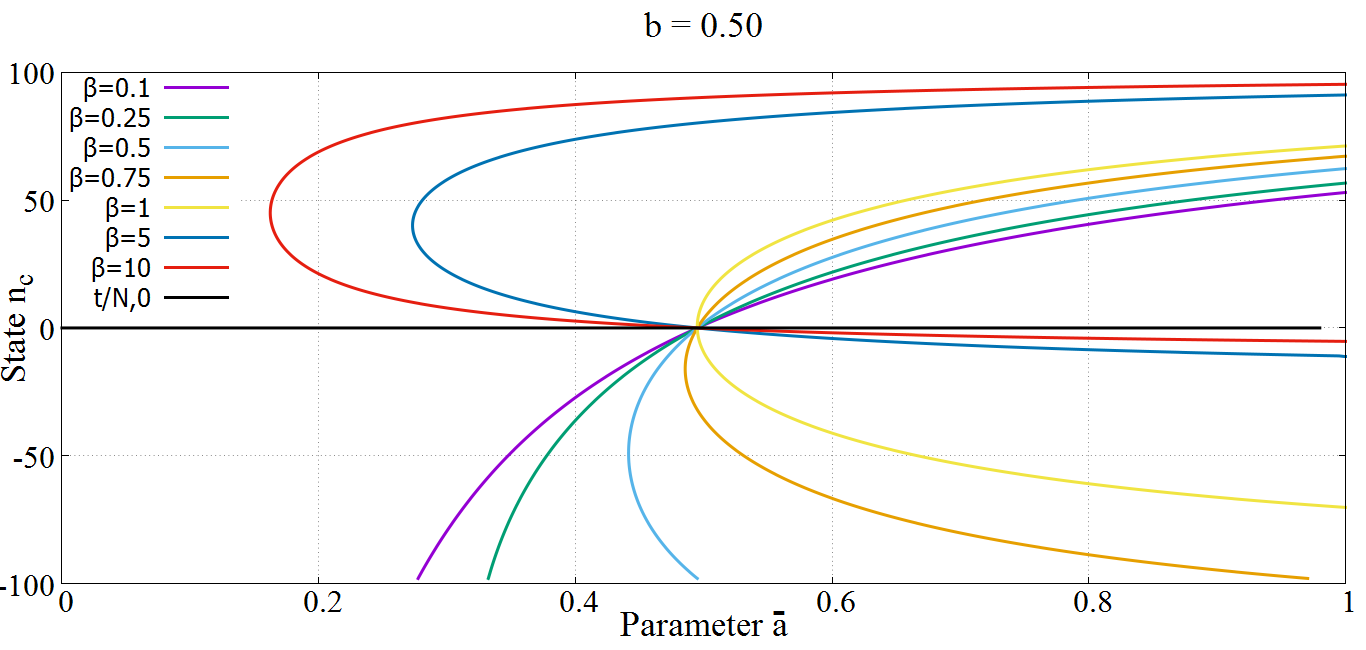
\includegraphics[width=\linewidth]{images/chapter3/phaseSpace.png}
  \caption{The phase space plot of the steady-state value $n_{c}$ versus $\bar{a}$ for various $\beta$ values and $b = 0.5$. Included is the trivial steaty-state solution $n_{c} = 0$}
  \label{fig:phaseSpace}
\end{figure}



\subsection{Critical Points}

From observing all phase space plots of various $b$ values, all $\beta$ curves intersect, along with the trivial solution, at a specific point.
Setting $n_{c} = 0$ in \eqref{eq:steadystate} gives us this critical point of intersection, $\bar{a}_{1}$:

\begin{equation}
\bar{a}_{1} = \frac{b(N-1)}{N}
\end{equation}

which for $N\gg1$ results to the observed $\bar{a}_{1}\approx b$. Solution for the critical point is shown in the appendix (\ref{apndx:crita1}

The non-trivial solution to the steady-state equation \eqref{eq:steadystate} is quadratic, which does not include the trivial solution.
This results to two non-trivial $n_{c}$ solutions for a given $\bar{a}$.
For $\beta\leq1$, the non-trivial steady-state solutions appear uniquely for $\bar{a}>\bar{a}_{1}$ since the second $n_{c}$ value is negative and therefore, extraneous.
However, when $\beta>1$, two non-trivial solutions appear between a new critical value of $\bar{a}=\bar{a}_{2}$, corresponding to the vertex of \eqref{eq:steadystate}, and $\bar{a}_{1}$.
For $\bar{a}>\bar{a}_{1}$, the non-trivial steady-state solution appears uniquely once again, similar to $\beta\leq1$.
The $\bar{a}_{2}$ is given by

\begin{equation}
\bar{a}_{2} = \frac{b(N-1)^{2}}{(N-n_{c}^{*})(N-1+\beta n_{c}^{*})}
\end{equation}

where $n_{c}^{*} \equiv [1+(\beta-1)N]/2\beta$.
Derivation is shown in the appendix (\ref{apndx:crita1}
This non-trivial solution however, is unstable upon substitution with $\ddot{\vec{n}}$ resulting to $\ddot{\vec{n}}<0$.
Thus, the middle branch in the range $\bar{a}\in(\bar{a}_{2},\bar{a}_{1})$ is an unstable steady-state.
%For $\bar{a} \geq b$, $n_{c}$ has three solutions: the trivial solution $n_{c}=0$ and the two solutions provided by \eqref{eq:steadystate}.
%For certain $\bar{a} < b$ values, a second, non-trivial solution appears.
 
\section{Simulation experiments}
\hspace{\parindent} Analytical results are confirmed by simulation. The number of iterations, $t$, is set to be much greater than the duration of the forcing function,$\tau$.
Figure~\ref{fig:compareSingleSS} shows sample simulations along with the analytical steady-state and the average of the system.
The analytical steady-state is plotted in green while the mean is plotted in red.
As observed, the simulation closely resembles the analytical value. The system settles to its steady-state very early in the simulation.
It can be safely assumed that the $n_{c}$ values at $t \gg \tau$ are equivalent to $n_{c}$ for $t \rightarrow \infty$.

\begin{figure}[h]
  \centering
  \begin{subfigure}[b]{0.4\linewidth}
    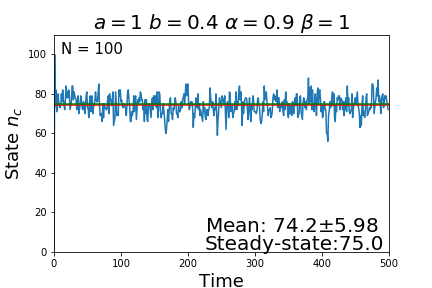
\includegraphics[width=\linewidth]{images/chapter3/ssA.png}
    \caption{A simulation with a non-trivial steady state of 75. The average $n_{c}$ is close to the analytic value.}
  \end{subfigure}
  \begin{subfigure}[b]{0.4\linewidth}
    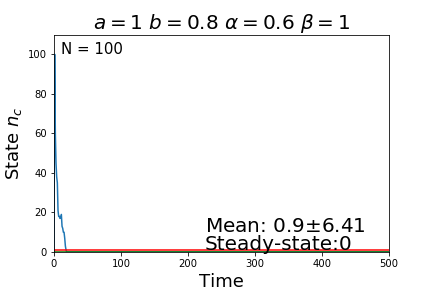
\includegraphics[width=\linewidth]{images/chapter3/ssB.png}
    %\label{fig:nonTrivSim}
    \caption{A simulation with a trivial steady state of 75. The average $n_{c}$ value is approximately $0$.}
  \end{subfigure}
  \caption{Sample simulations that compare the analytical steady-state of the given parameters and the mean $n_{c}$ value of the system.}
  \label{fig:compareSingleSS}
\end{figure}

$10$ sample runs were performed with different initial random number generator states and the final $n_{c}$ value for each iteration were recorded.
The mean and standard deviation of the simulated steady-state values are then computed for each parameter space $(\bar{a},b,\beta)$. 
The data points were then plotted with the corresponding parametrized differential curve shown in Fig.~\ref{fig:phase+sim}.
All code used is provided in the appendix (\ref{apndx:steadstatesim}), as well as more simulation experiments for various $b$ values (\ref{apndx:ssexpt}

\begin{figure}[h!]
 \centering
  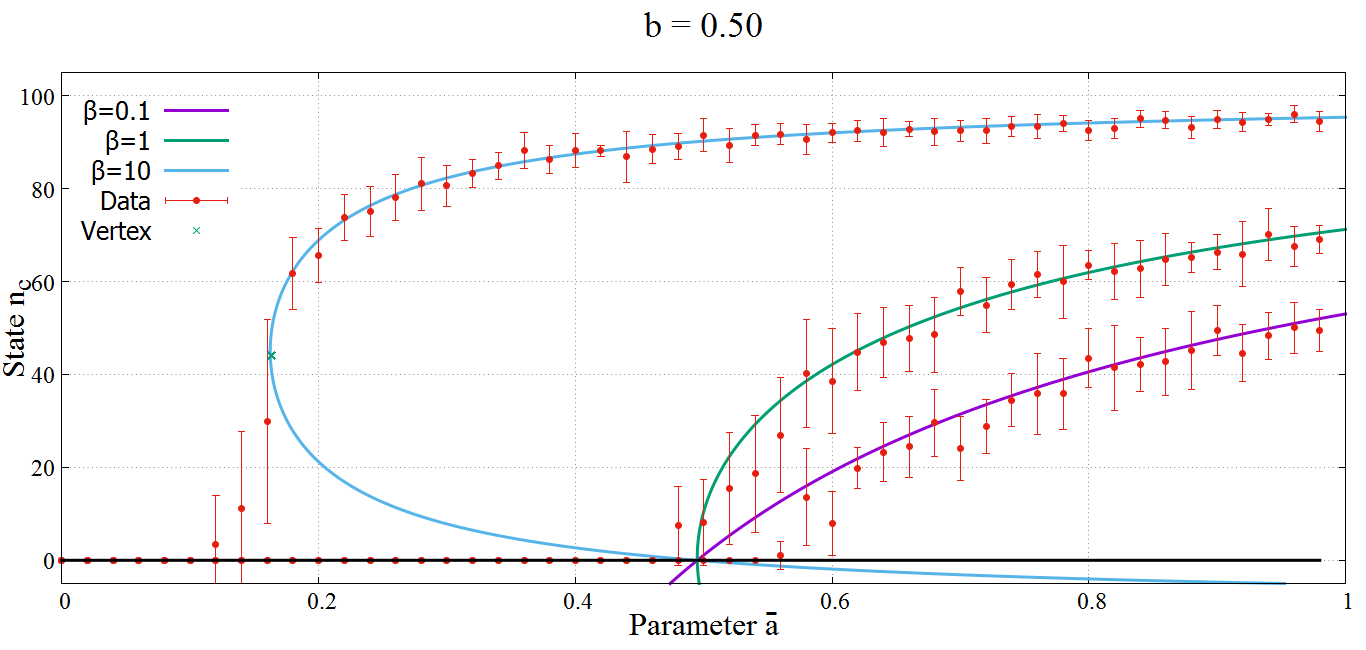
\includegraphics[width=\linewidth]{images/chapter3/phase+sim.png}
  \caption{The simulated steady-state values plotted against the analytic steady-state curves. The error bars provide the extent of deviation in simulations. The vertex is represented with the cross.}
  \label{fig:phase+sim}
\end{figure}

For $\beta \leq 1$, the simulation is consistent with the trivial steady state solution until it reaches the critical point $\bar{a} = b$, after which follows non-trivial, non-extraneous solution consistent with \eqref{eq:steadystate}.
For $\beta > 1$, the simulation follows the trivial steady-state and then breaks away and approaches the vertex of \eqref{eq:steadystate} at $\bar{a}_{2}$, after which, continues to follow the upper branch of \eqref{eq:steadystate}.
The analytical solutions fail to predict the bifurcation from the trivial solution to the vertex of the curve.
Also, the significance of the lower branch for $\beta > 1$ curves is unknown and warrants further investigation.
The vertex is said to be unstable due to the fact that it unreliably and unpredictably settles to either trivial or non-trivial solution.
The lower branch may share this instability.    

\subsection{Unstable points}
For the previous simulation experiments, all agents start at state S and then forced to transition to state C. 
To investigate the properties of the lower branch on the non-trivial solution, we vary the number of agents that start the simulation in state C and remove the forcing function. 
This allows us to determine where the system will settle given the specific starting $n_{c}$ value, more particularly for $n_{c}$ values near the lower branch of the non-trivial solution. 
The code that generate the vector graphs is provided in the appendix (\ref{apndx:vectsim})

Shown in figure \ref{fig:compareSingleSS} are the new phase space graphs that include arrows that point to where that $n_{c}$ value for the given $\bar{a}$ settles.
More vector graphs are available in the appendix (\ref{apndx:vectgraph}
The color of the arrows represents the probability of going towards that direction.
Intuitively for $\beta \leq 1$, all $n_{c}$ values point towards the trivial solution for all $\bar{a}$ values less than  $\bar{a}_{1}$. 
All $n_{c}$ with $\bar{a}$ values greater than $\bar{a}_{1}$ point towards the non-trival solution.
For $\beta > 1$, what differs is the behavior at the vertex and the lower branch of the non-trivial solution.
$n_{c}$ values above the vertex have an estimated 50\% to either settle at the vertex or zero, while $n_{c}$ values below the vertex absolutely settle to zero.
Points slightly above the lower branch tend more towards settling to the upper branch but still have a chance to settle at 0.
Likewise for points below the lower branch.
Points within the lower branch have a 50\% of settling to either trivial or non trivial solution.

\begin{figure}[h!]
 \centering
  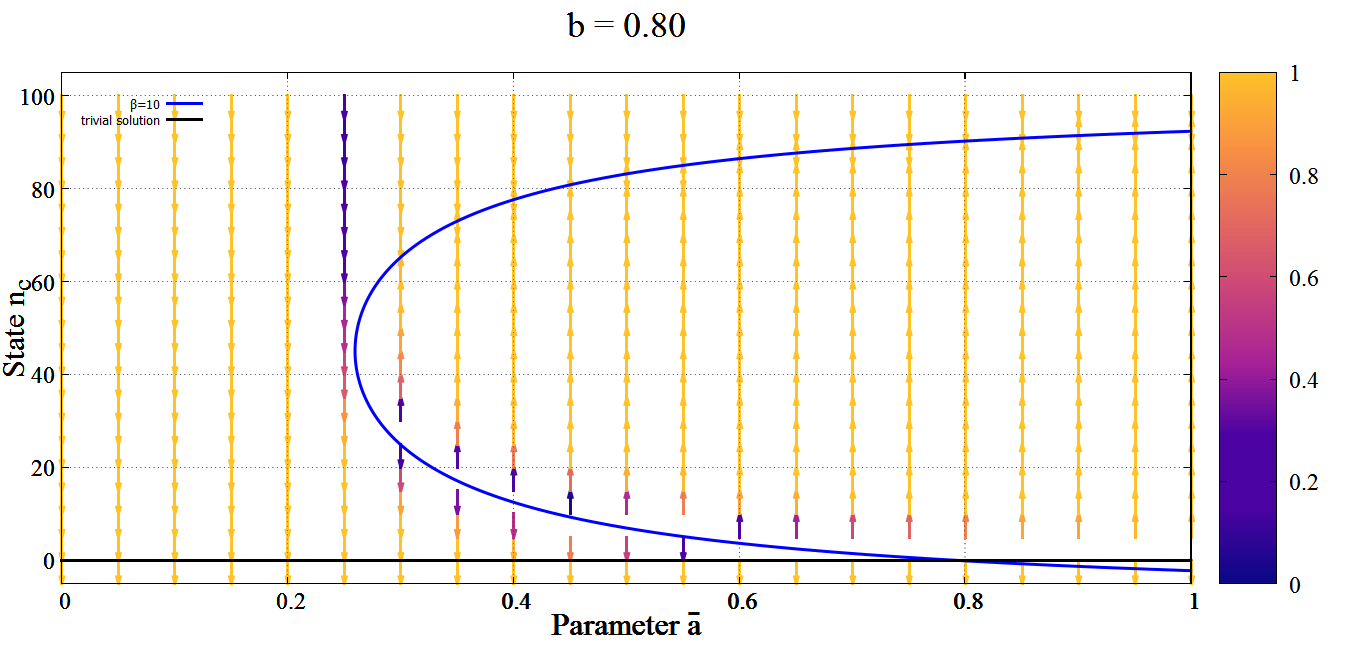
\includegraphics[width=\linewidth]{images/appendix/vectors/4.png}
  \caption{Vector graph for parameters $b = 0.8, \beta = 10$. The origin of the vector represents the initial $n_{c}$ and corresponding $\bar{a}$ value. The direction it points reveals whether it settles to the trivial or non-trivial solution. The color represents the probability of settling towards the directed steady-state.}
  \label{fig:compareSingleSS}
\end{figure}

%%

%\begin{figure}[htb]
%\centering
%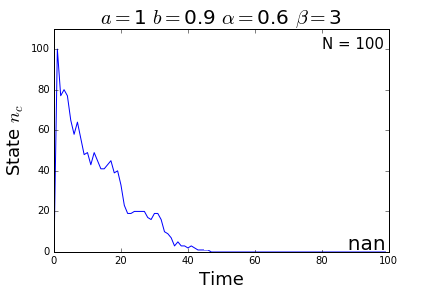
\includegraphics[width=0.3\columnwidth]{simulation/sim1}
%\includegraphics[width=0.3\columnwidth]{simulation/sim2}
%\includegraphics[width=0.6\columnwidth]{sim2}
%\caption{
%Sample simulations for $N = 100$ with the parameters: (a) $\bar{a} = 0.6$, $b = 0.9$ and $\beta = 3$ and (b) $\bar{a} = 0.36$, $b=0.7$ and $\beta = 14$.
%The simulation in (a) settles to the trivial steady-state ($n_{c}=0$) while the results in (b) show an average of $\langle{n_{c}}\rangle\approx85.5\pm 9.53$.
%[!! Remove the labels ``Steady State: ...''. One does not report an average with too many significant digits. What is the actual standard deviation (SD) here? Keep the decimal digits of the reported SD to two maximum.]
%(c) The average of the simulated steady-state values for different parameters are shown together with the theoretical predictions.
%The error bars provide the extent of the sample standard deviations computed. The cross indicates the vertex given by (9), i.e., $\bar{a_{2}}$
%} \label{fig:parametric}
%\end{figure}









\chapter{Incorporating Spatial Effects}
\label{chap4}

\hspace{\parindent} After analysing the model, it was then compared to real applause.
The applause duration of varying audience sizes were taken from Youtube videos of musical concerts and performances.
The applause duration was manually recorded.
The audience size was either taken from the seating capacity and/or ticket sales for the given concert/performance, or was estimated by the area or room the audience resided in.
The relationship of the data set was tested with both applause duration and population size in order to find an appropriate linear dependence, as shown in figure \ref{fig:realclap}.

\begin{figure}[h]
  \centering
  \begin{subfigure}[b]{0.4\linewidth}
    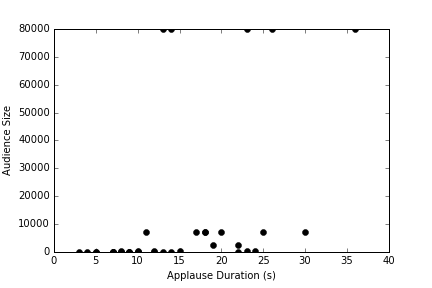
\includegraphics[width=\linewidth]{images/chapter4/1.png}
    \caption{Graphing size versus applause duration.}
  \end{subfigure}
  \begin{subfigure}[b]{0.4\linewidth}
    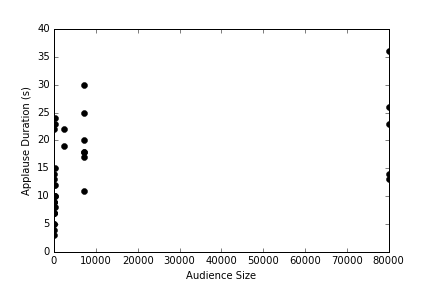
\includegraphics[width=\linewidth]{images/chapter4/2.png}
    \caption{Graphing applause duration versus size.}
  \end{subfigure}
    \begin{subfigure}[b]{0.4\linewidth}
    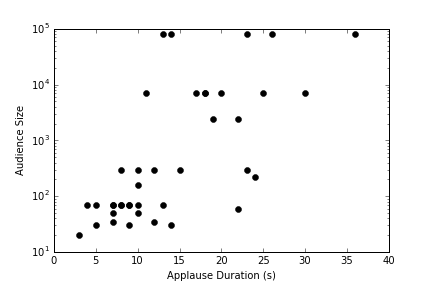
\includegraphics[width=\linewidth]{images/chapter4/3.png}
    %\label{fig:nonTrivSim}
    \caption{Graphing size (in the logarithmic scale) versus applause duration}
  \end{subfigure}
    \begin{subfigure}[b]{0.4\linewidth}
    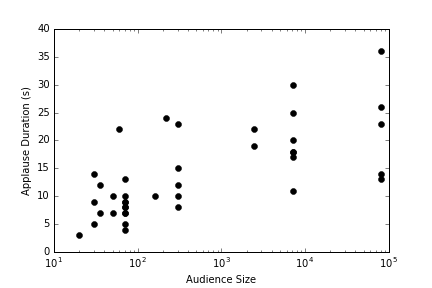
\includegraphics[width=\linewidth]{images/chapter4/4.png}
    %\label{fig:nonTrivSim}
    \caption{Graphing applause duration versus size (in the logarithmic scale).}
  \end{subfigure}
  \caption{Different graphs of the data points of real-life applause.}
  \label{fig:realclap}
\end{figure}

Figure \ref{fig:realclap} (d) makes the most sense; the applause duration of the audience is dependent on the size of the audience.
The question now is whether or not the compartmental model can recreate \ref{fig:realclap} (d).
The current model shows no population size dependence; changing the population size does not affect the applause duration for a given set of parameters.
This is because of the assumption that the network is fully connected, meaning that an audience member in front is influenced the exact same way by the whole audience as an audience member at the back.
As this does not seem to be the case in real-life applause, spatial effects must be incorporated by modifying the feedback function $f'(\alpha)$.

\section{Different configurations for field of vision}

\hspace{\parindent}The field of view configurations represent the audience members that may influence the reference agent.
In real life, the  reference agent is influenced by a limited number of audience members, not the whole audience.
The network is no longer fully-connected, observing a modified, extended Moore neighborhood.
It is extended since it considers all agents till the front row of the system, and not just those $1$ unit away.
It is modified since it does not consider all directions; the directions considered are affected by the configuration.
$\theta = 0$ represents all audience members only directly in front of the reference agent until the very front. 
$\theta = \pi$ represents all rows ahead of the reference agent. 
$\theta = \frac{\pi}{2}$ considers all agents from the north-east direction to the north-west in a $90$ degree arc. The configurations are shown in figure \ref{fig:spaceconfig}.

\begin{figure}[h]
  \centering
  \begin{subfigure}[b]{0.3\linewidth}
    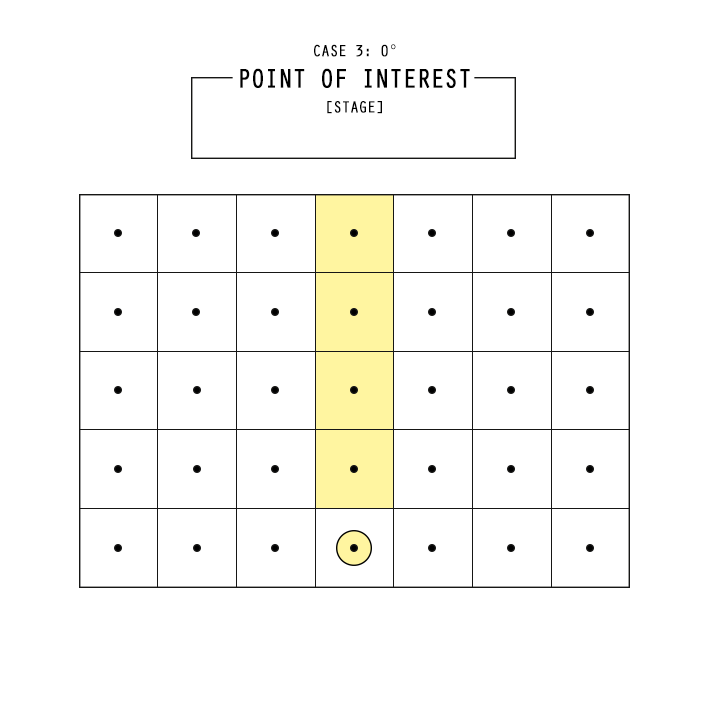
\includegraphics[width=\linewidth]{images/chapter4/0degD.png}
    \caption{$\theta = 0$}
  \end{subfigure}
  \begin{subfigure}[b]{0.3\linewidth}
    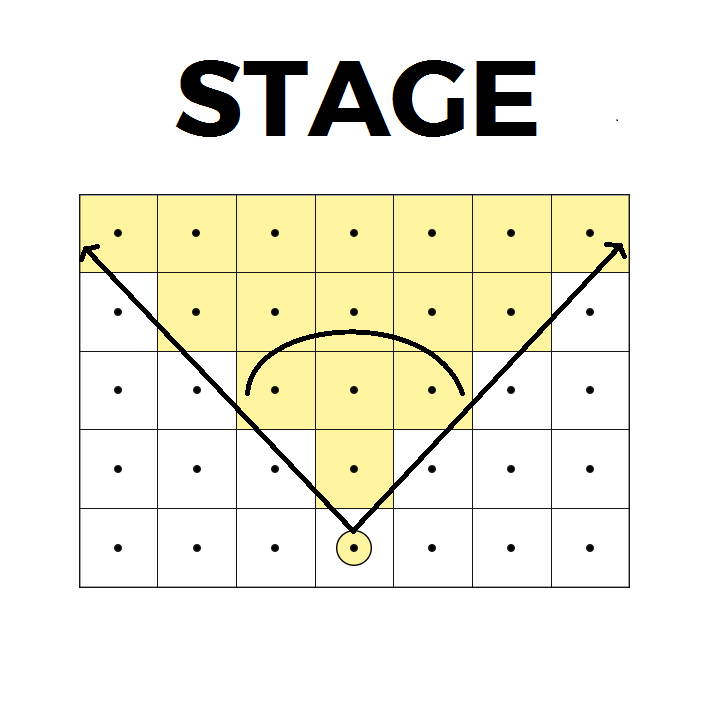
\includegraphics[width=\linewidth]{images/chapter4/90degD.png}
    \caption{$\theta = \frac{\pi}{2}$}
  \end{subfigure}
    \begin{subfigure}[b]{0.3\linewidth}
    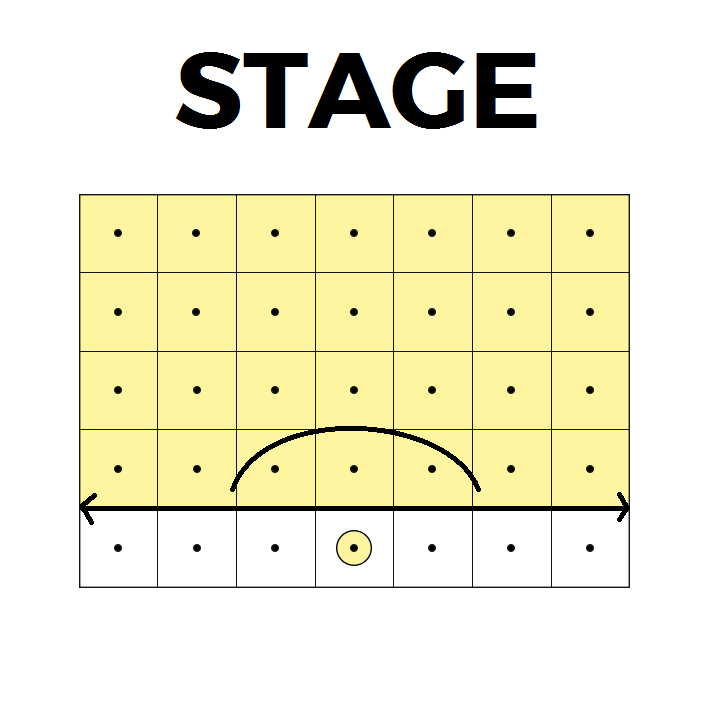
\includegraphics[width=\linewidth]{images/chapter4/180degD.png}
    %\label{fig:nonTrivSim}
    \caption{$\theta = \pi$}
  \end{subfigure}
  \caption{Different field-of-view configurations. The encircled black dot shaded in yellow is the reference agent. The boxes highlighted in yellow are what can influence the  encircled reference agent.}
  \label{fig:spaceconfig}
\end{figure}

\section{Simulating the different spatial configurations}

\hspace{\parindent} Initially, $f'(\alpha)$ bases the fraction of $n_{c}$ throughout the whole population. After incorporating spatial effects, that fraction is only within the field-of-view of the reference agent.
The feedback function is still parametrized by $\alpha$.
%The code developed is provided in Appendix \ref{apndx:spacesim}.

\begin{figure}[h]
  \centering
  \begin{subfigure}[b]{0.4\linewidth}
    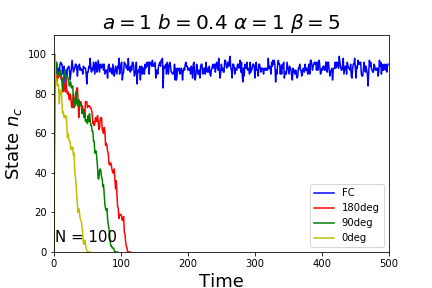
\includegraphics[width=\linewidth]{images/chapter4/feedback_sim4.png}
    \caption{Comparing simulations with spatial effects to the original fully-connected simulation.}
  \end{subfigure}
  \begin{subfigure}[b]{0.4\linewidth}
    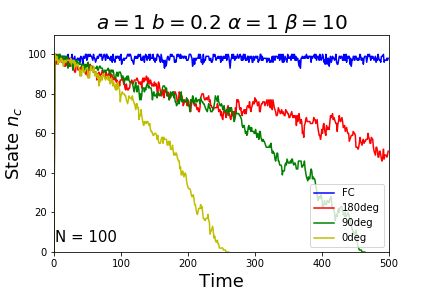
\includegraphics[width=\linewidth]{images/chapter4/feedback_sim5.png}
    \caption{$\theta = 180$ has yet to reach steady-state but is steadily heading towards $0$.}
  \end{subfigure}
    \begin{subfigure}[b]{0.4\linewidth}
    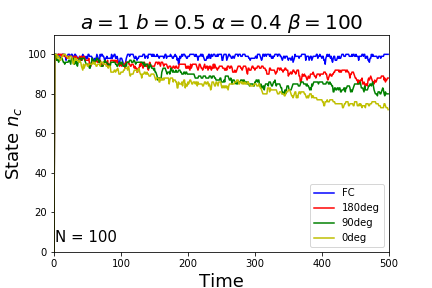
\includegraphics[width=\linewidth]{images/chapter4/feedback_sim6.png}
    %\label{fig:nonTrivSim}
    \caption{All simulations are slowly reaching steady-state.}
  \end{subfigure}
    \begin{subfigure}[b]{0.4\linewidth}
    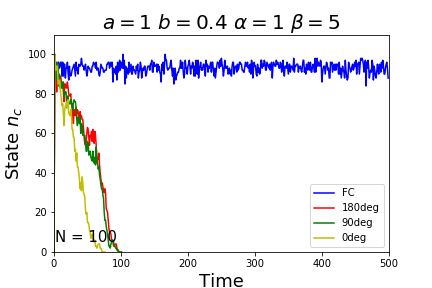
\includegraphics[width=\linewidth]{images/chapter4/feedback_sim3.png}
    %\label{fig:nonTrivSim}
    \caption{A case where $\theta = \frac{\pi}{2}$ is similar to $\theta = 0$.}
  \end{subfigure}
    \begin{subfigure}[b]{0.4\linewidth}
    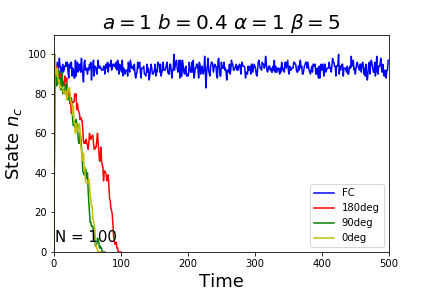
\includegraphics[width=\linewidth]{images/chapter4/feedback_sim2.png}
    %\label{fig:nonTrivSim}
    \caption{A case where $\theta = \frac{\pi}{2}$ is similar to $\theta = \pi$.}
  \end{subfigure}
  \begin{subfigure}[b]{0.4\linewidth}
    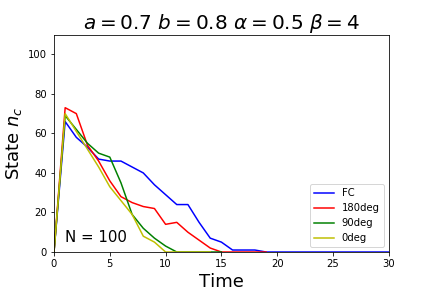
\includegraphics[width=\linewidth]{images/chapter4/feedback_sim7.png}
    %\label{fig:nonTrivSim}
    \caption{All configurations have a trivial steady-state $0$.}
  \end{subfigure}
  \caption{Different graphs comparing effect of different feedback functions under different parameters.}
  \label{fig:spacesim}
\end{figure}

Shown in figure \ref{fig:spacesim} are simulations with different parameters ($a,b,\alpha,\beta$) comparing the different feedback functions, the original fully-connected network, $\theta = \pi$, $\theta = \frac{\pi}{2}$, and $\theta = 0$.
Graphs (a), (b), and (c) show that in our system, feedback functions are less effective in less connected networks. 
There is clearly a downward trend when it comes to applause duration.
Graphs (d) and (e) show that $\theta = \frac{\pi}{2}$ can be similar to either remaining configurations, as well as be somewhere in between.
Generally, simulations incorporating any form of field-of-view feedback do not have a non-trivial steady-state.
Graphs (b) and (c) show cases where the simulations have not ended, but exhibit an obvious downward trend.
Given more iterations, the simulations would end, unlike the fully-connected ones.
Graph (g) shows a special case where all simulations have a trivial steady-state of zero.
One thing to note is that the analysis done for the fully-connected system (phase space graphs, critical and unstable points) cannot be applied to the systems with spatial effects.
A different steady-state equation must be setup to reflect how each agent is influenced differently.
Such analysis will no longer be pursued as it is outside the scope of the study.

\section{Finding the parameters $(a,b,\alpha,\beta)$ for real-life applause}

\hspace{\parindent}Recalling, incorporating spatial effects to the feedback function effectively reduces the number of agents influencing a reference agent. Increasing the population size should increase the feedback since the agents in the back row of a 100x100 grid should 'see' more people than those in the back row of a 10x10 grid. 
This effectively eliminates the original problem of the fully-connected network being scale free.
It is now possible for the applause duration to be dependent on the population.
This phenomena is investigated by simulating a set of parameters $(a,b,\alpha,\beta)$ with varying populations.
For simplicity, the system grid will always be a 2-dimensional lattice of equal lengths.
Also, the spatial configuration used will be $\theta = \pi$.
The total population sample will be perfect squares ranging from $10^1$ to $10^4$.

%The code developed is provided in Appendix \ref{apndx:popdep}.

For this case, each iteration is considered  $1$ second.
Five trials were performed per sample population.
Due to insufferable run times, if a parameter set $(a,b,\alpha,\beta,N)$ returned a trial with applause duration greater than $60$ seconds, it is marked as $0$ seconds and no further trials are performed.
This means that graphs with data points of $0$ seconds are to be disregarded.

\begin{figure}[h]
  \centering
  \begin{subfigure}[b]{\linewidth}
    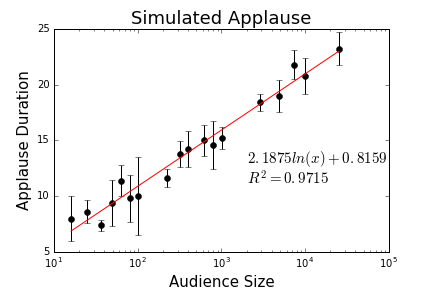
\includegraphics[width=\linewidth]{images/chapter4/sim.png}
    \caption{Simulated points showing population size dependence.}
  \end{subfigure}
  \begin{subfigure}[b]{\linewidth}
    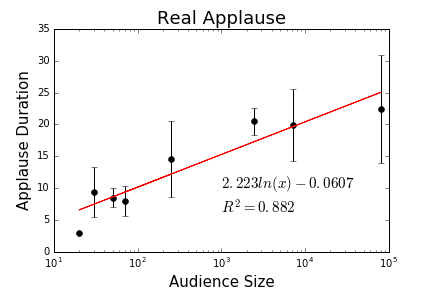
\includegraphics[width=\linewidth]{images/chapter4/real.png}
    \caption{Real-life data points on population size dependence.}
  \end{subfigure}
  \caption{Comparing the simulated and actual graph of applause duration versus population size. Both increase linearly in the logarithmic scale.}
  \label{fig:durXsizComp}
\end{figure}

Shown in figure \ref{fig:durXsizComp} is the parameter set $(a=1,b-0.7,\alpha=0.8,\beta=1)$ that best recreates the real-life applause. 
This was found by simply generating the applause duration versus audience size graph for every parameter set, then comparing its fitting function with that of the real applause. 
Similar parameter sets are shown in the appendix (\ref{apndx:bestfit})
Though this is the best fit parameter set, it still does not fully emulate the real applause.
As seen, the data points for the real-life applause is more deviant compared to the simulation.
The model may still be incomplete, or the data points for real-life applause is not enough.
On reason for this is that the data points for real applause is not enough.
Data acquisition was difficult due to a duration-size uncertainty.
For big audience sizes, the size is well defined because of the seating capacity of the stadium or the ticket sales for the event. 
Applause duration is very uncertain because it is very hard to determine when the applause starts and ends due to the sheer amount of people.
Also, at no point does the crowd go completely silent, making it hard to distinguish applause from cheers and screems.
For small audience sizes, the applause is well defined since it is clearly audible in the video, and can also be visually confirmed.
The audience size is uncertain because the videos of small audience sizes are either street performances or room performances.
For street perfomances, people come and go.
For room performances, the videographer is focused on the performer, thus the audience size cannot be confirmed with absolute certainty and must be estimated.
Another source for error is the spatial configuration. 
The given setup only accounts for sight. A box with the reference agent at the center can be added in order to account for audible influence.
Finally, the assumption that everyone claps after the performance does not encapsulate all forms of audience applause.
This aspect can included by varying the forcing function to different probabilities, instead of 100%.
An in-depth analysis on the new model is also warranted.


\chapter{Conclusions and Recommendations}
\label{conclusions}

\hspace{\parindent} In this thesis, we have reviewed the definition of the revival time associated with the wave packet revival phenomena. We have obtained approximate analytical expressions for the classical time scale $T_{cl}$ and quantum revival time scale $T_{rev}$ for the single- and double- $\delta$-perturbed infinite square well system.




%% include your appendix here AFTER the entire contents..
\appendix \chapter{Appendix}
\label{appendix}

\section{Combined probability of functions $f$ and $f'$}
\label{apndx:prob}

\hspace{\parindent} The forcing function $f$ permits agents to undergo $\mathrm{R_{1}}$ and is represented with a probability $p_{1}$.
The probability that $\mathrm{R_{1}}$ does not occur is $q_{1} = 1 - p_{1}$.
Likewise for the function $f'$ to undergo $\mathrm{R_{1}}$ is represented with a probability $p_{2}$, and non-occurring probability $q_{2}$.
Combining the probabilities $p$ and $q$ results to

\begin{eqnarray}
\label{eqn:conservP1}
p_{1} + q_{1} &&= 1 \\
\label{eqn:conservP2}
p_{2} + q_{2} &&= 1
\end{eqnarray}

Multiplying the equations \eqref{eqn:conservP1} and \eqref{eqn:conservP2} and simplifying

\begin{eqnarray}
(p_{1} + q_{1})(p_{2} + q_{2}) &&= 1 \\
p_{1}p_{2} + p_{1}q_{2} + p_{2}q_{1} + q_{1}q_{2} &&= 1
\end{eqnarray}

$q_{1}q_{2}$ represents neither event occuring thus

\begin{eqnarray}
p_{net} = 1 - q_{1}q_{2} &&= 1 - (1-p_{1})(1-p_{2}) \\
&&= 1 - (1 - p_{1} - p_{2} + p_{1}p_{2}) \\
&&= p_{1} + p_{2} - p_{1}p_{2}
\label{apndx:simpleProb}
\end{eqnarray}

Replacing \eqref{eq:simpleProb} with the functions gives
\begin{equation}
p_{net} = f + f' - f'f
\end{equation}
which is used in \eqref{eq:p(r1)}

\newpage
\section{Library of applause functions}
\label{apndx:codelib}
\begin{lstlisting}

from random import random
from numpy import zeros, sqrt, sum, nan_to_num
from math import isnan

#function that forces agents to go to state C
def force_func(t, end):
    if t < end:
        return 1
    else:
        return 0

#f'(alpha); feedback based on the number of ppl already in state C; the more ppl in state C, the more ppl will clap
def feedback_alpha(alpha, nC, population):
    return alpha * nC / (population - 1)
    
#g'(beta)
def feedback_beta(beta, nC, population):
    return 1 / (1 + beta * nC / (population - 1))
       
#spatial-dependent feedack, you can control the 'radius' of the reference agent
#taper refers to how many to add at the ends;radius = 0 taper = 1 is '90deg'    
def feedback_space(alpha,system,system_row, system_column, N, M, radius, taper):
    applause_state = []
    for i in range(system_row):
        radius_mech = 0
        applause_state.append(system[i,system_column])
        while radius_mech != radius + taper*(system_row - i):
            radius_mech += 1
            if system_column + radius_mech < M:
                applause_state.append(system[i,system_column + radius_mech])
            if system_column - radius_mech > -1:
                applause_state.append(system[i,system_column - radius_mech])
    return alpha*nan_to_num(sum(applause_state)/len(applause_state))
    
def feedback_180deg(alpha,system,system_row, M): #reverted to simpler feedback space functions since runs took too long
    applause_state = [0]
    for i in range(system_row):
        applause_state.append(sum(system[i]))
    return alpha*nan_to_num(sum(applause_state)/(system_row*M))    

#quadratic equation    
def quad_eq(x,y,z,sign):
    return (-y + sign * (sqrt((y ** 2) - 4 * x * z))) / 2 * x

#do i still need this??!?!
def frange(start, stop, step):
    i = start
    while i < stop:
        yield i
        i += step
   
#creates 'network' of audience        
def audience(N,M,C):
    agents = zeros((N,M))
    
    for i in range(N):
        for j in range(M):
            if sum(agents) == C:
                break
            else:
                agents[i][j]=1
    
    return agents

#the actual simulator            
def app_sim(aStoC, bCtoS, alpha, beta, N, M, C, t, t_1):
    population = N * M
    AGENT = audience(N, M, C)
    graph = []

    for k in range(t):
        nC = sum(AGENT) #number of people clapping
        graph.append(nC)
        for i in range(N):
            for j in range(M):
                if AGENT[i,j] == 0:
                    if random() <= aStoC * (1 - (1-force_func(k, t_1)) * (1 - feedback_alpha(alpha, nC, population))):
                        AGENT[i,j] += 1
                else:
                    if random() <= bCtoS * feedback_beta(beta, nC, population):
                        AGENT[i,j] -= 1
    return graph

#sim with spatial dependence specific to 180 deg
def sim_space(aStoC, bCtoS, alpha, beta, N, M, C, t, t_1):
    population = N * M
    AGENT = audience(N, M, C)
    graph = []
    zeroCount = 0

    for k in range(t):
        nC = sum(AGENT) #number of people clapping
        if nC == 0:
            zeroCount += 1
        graph.append(nC)
        for i in range(N):
            for j in range(M):
                if AGENT[i,j] == 0:
                    if random() <= aStoC * (1 - (1-force_func(k, t_1)) * (1 - feedback_180deg(alpha,AGENT,i, M))):
                        AGENT[i,j] += 1
                else:
                    if random() <= bCtoS * feedback_beta(beta, nC, population):
                        AGENT[i,j] -= 1
        if zeroCount == 6:
            break
            return graph
    return graph
 
#graphs theoretical steady_state based on parameters    
def steady_nC(aStoC, bCtoS, alpha, beta, population, sign):
    if beta == 0:
        if alpha == 0:
            return (aStoC * population) / (aStoC+bCtoS)
        else:
            if sign == 1:
                return population - (bCtoS * (population - 1)) / (aStoC * alpha)
            else:
                return 0
    else:
        if alpha == 0:
            return 0
        else:
            if sign == 0:
                return 0
            else:
                if isnan(quad_eq(1, ((population*aStoC*alpha*beta)-(population*aStoC*alpha)+(aStoC*alpha))/(-aStoC*alpha*beta), (((population**2)*aStoC*alpha) - (population*aStoC*alpha) - ((population**2)*bCtoS) + (2*population*bCtoS) - (bCtoS))/(-aStoC*alpha*beta), sign)) == True:
                    return 0
                else:
                    return quad_eq(1, ((population*aStoC*alpha*beta)-(population*aStoC*alpha)+(aStoC*alpha))/(-aStoC*alpha*beta), (((population**2)*aStoC*alpha) - (population*aStoC*alpha) - ((population**2)*bCtoS) + (2*population*bCtoS) - (bCtoS))/(-aStoC*alpha*beta), sign)

\end{lstlisting}

\newpage
\section{Deriving the steady-state equation}
\label{apndx:derivSS}
\hspace{\parindent} Setting $\frac{d\vec{n}}{dt} = 0$,

\begin{align}
\frac{d}{dt}n_{c} & = 0\\
a(f+f'-f'f)n_{s} - bg'n_{c} & = 0\\
a(f+f'-f'f)n_{s} & = bg'n_{c} \\
\end{align}

Note: $N = n_{c} + n_{s}, n_{s} = N - n{c}$, and $f = 0$.

\begin{equation}
af'(N - n{c}) = bg'n_{c} \\
\label{eq:noFunc}
\end{equation}

Plugging in \eqref{eq:f'} and \eqref{eq:g'} to \eqref{eq:noFunc}:

\begin{align}
a(\alpha\frac{n_{c}}{N-1})(N - n_{c}) &= b(\frac{1}{1 + \frac{\beta n_{c}}{N-1}})(n_{c}) \\
\frac{a\alpha (N - n_{c})}{N-1}n_{c} &= b\frac{N-1}{N-1+\beta n_{c}}n_{c} \\
a\alpha (N - n_{c}) &= b\frac{(N-1)^2}{N-1+\beta n_{c}} \\
a\alpha(N-n_{c})(N-1 + \beta n_{c}) & = b(N-1)^{2}
\end{align}

\newpage
\section{Steady-state Phase Space}
\label{apndx:phaseSpace}
\hspace{\parindent} Shown are the phase space plots for various $b$ values.
\begin{figure}[h!]
 \centering
  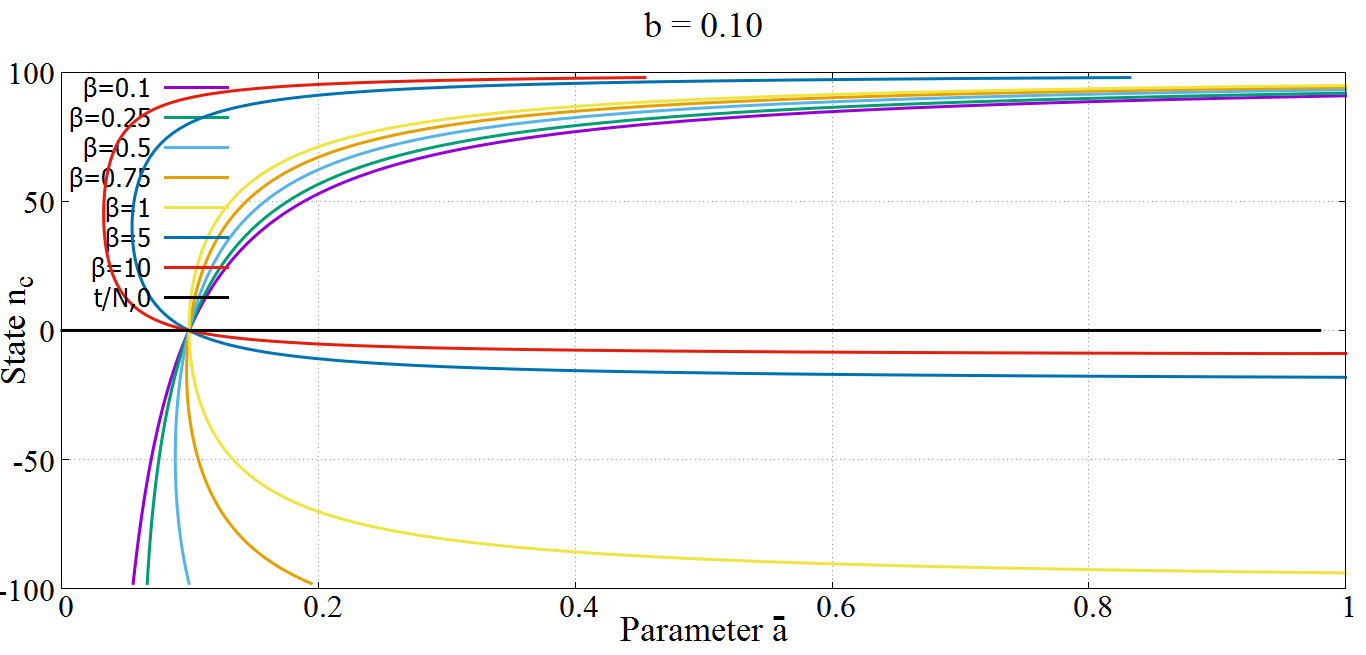
\includegraphics[width=\linewidth]{images/appendix/phaseSpace/1.png}
\end{figure}

\begin{figure}[h!]
 \centering
  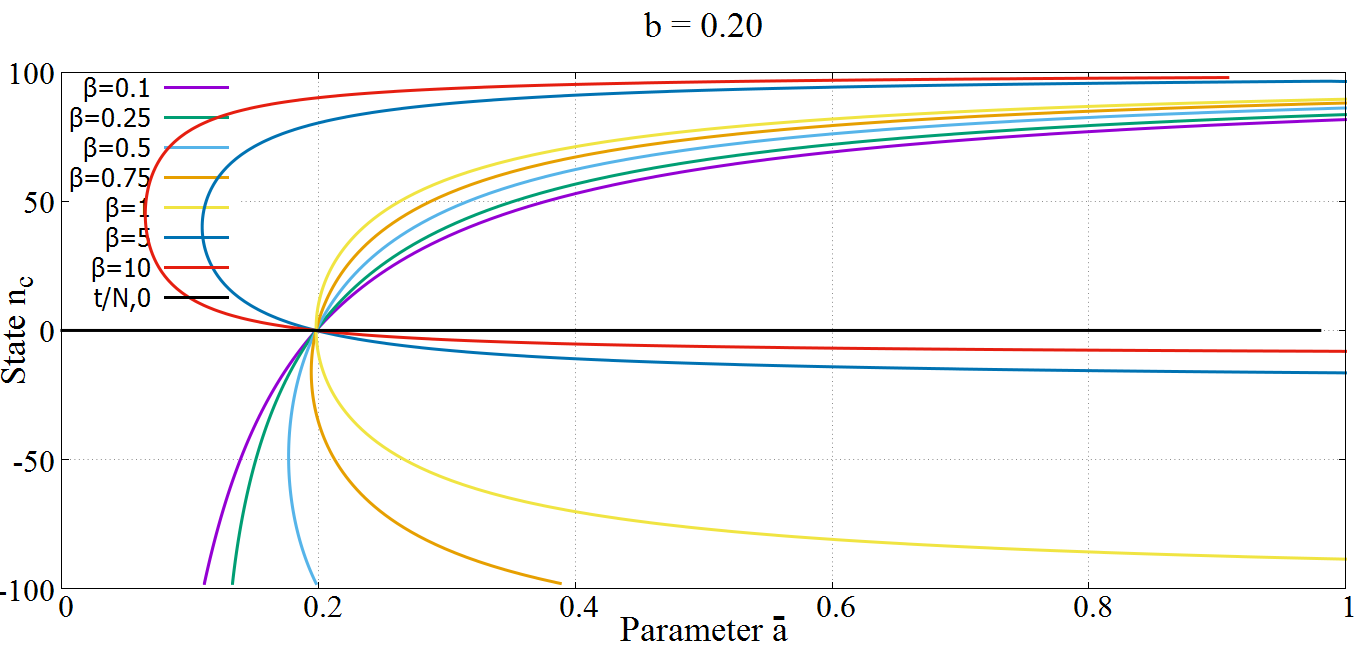
\includegraphics[width=\linewidth]{images/appendix/phaseSpace/2.png}
\end{figure}

\begin{figure}[h!]
 \centering
  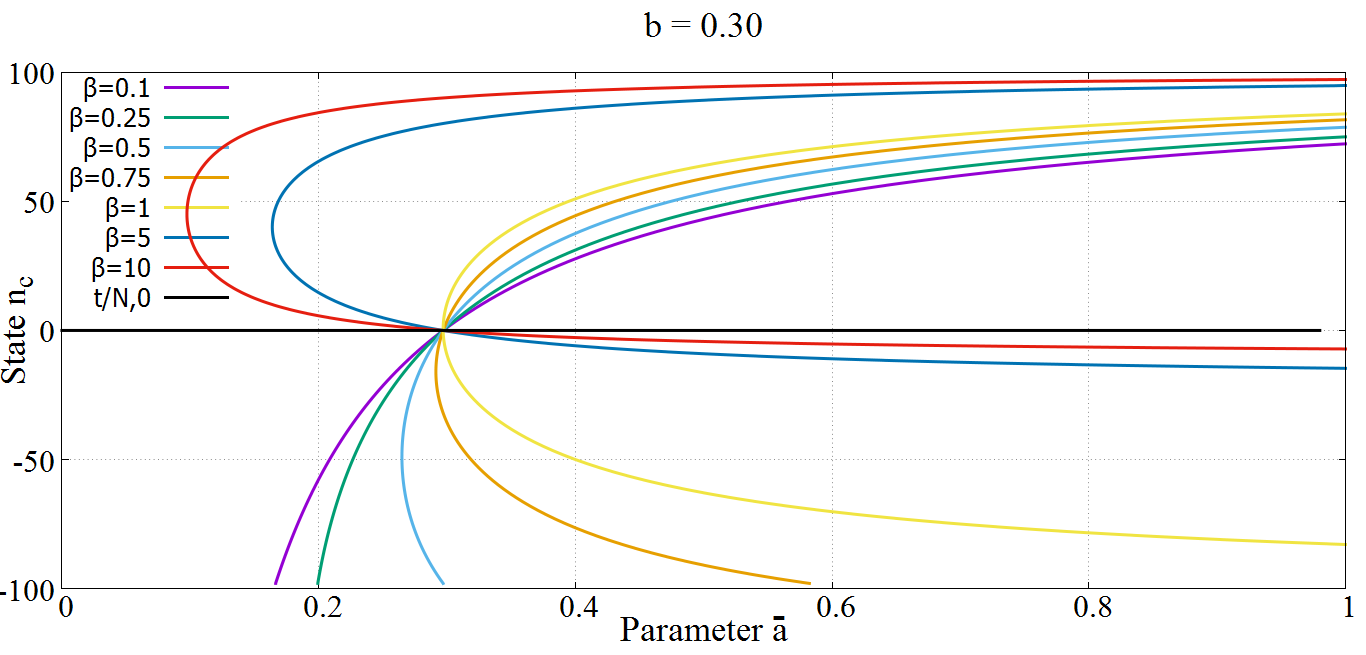
\includegraphics[width=\linewidth]{images/appendix/phaseSpace/3.png}
\end{figure}
\newpage
\begin{figure}[h!]
 \centering
  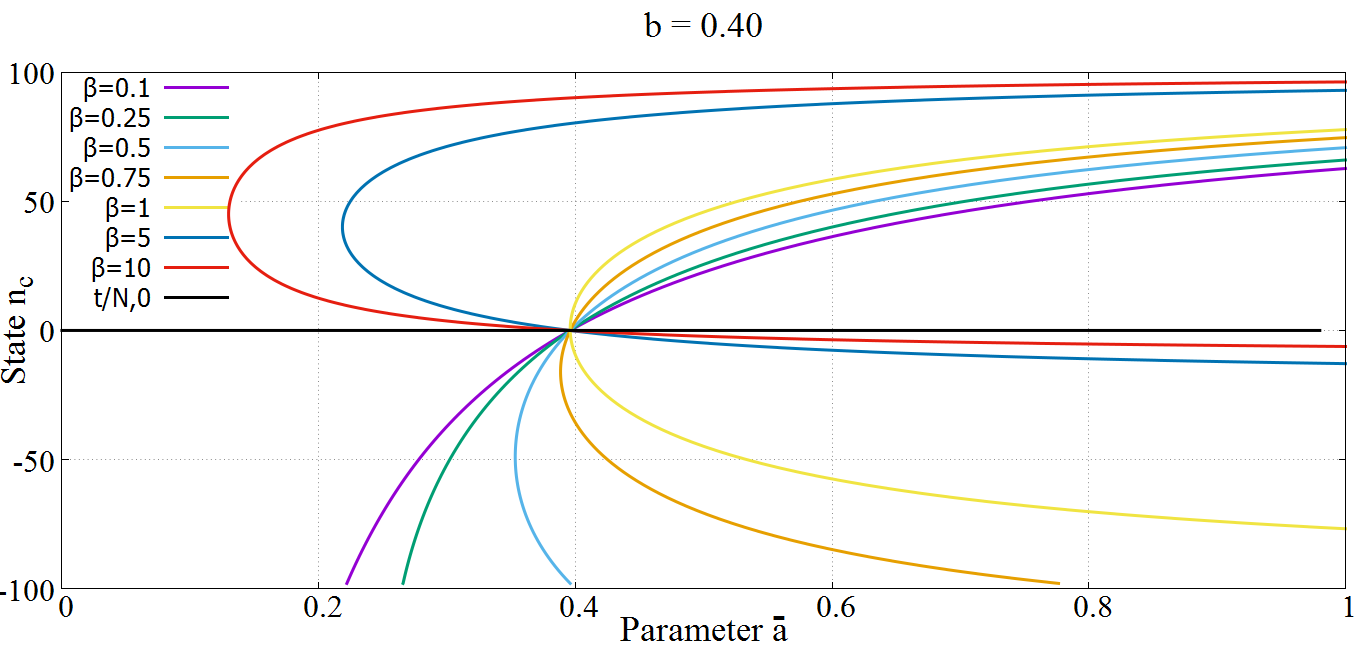
\includegraphics[width=\linewidth]{images/appendix/phaseSpace/4.png}
\end{figure}
\newpage
\begin{figure}[h!]
 \centering
  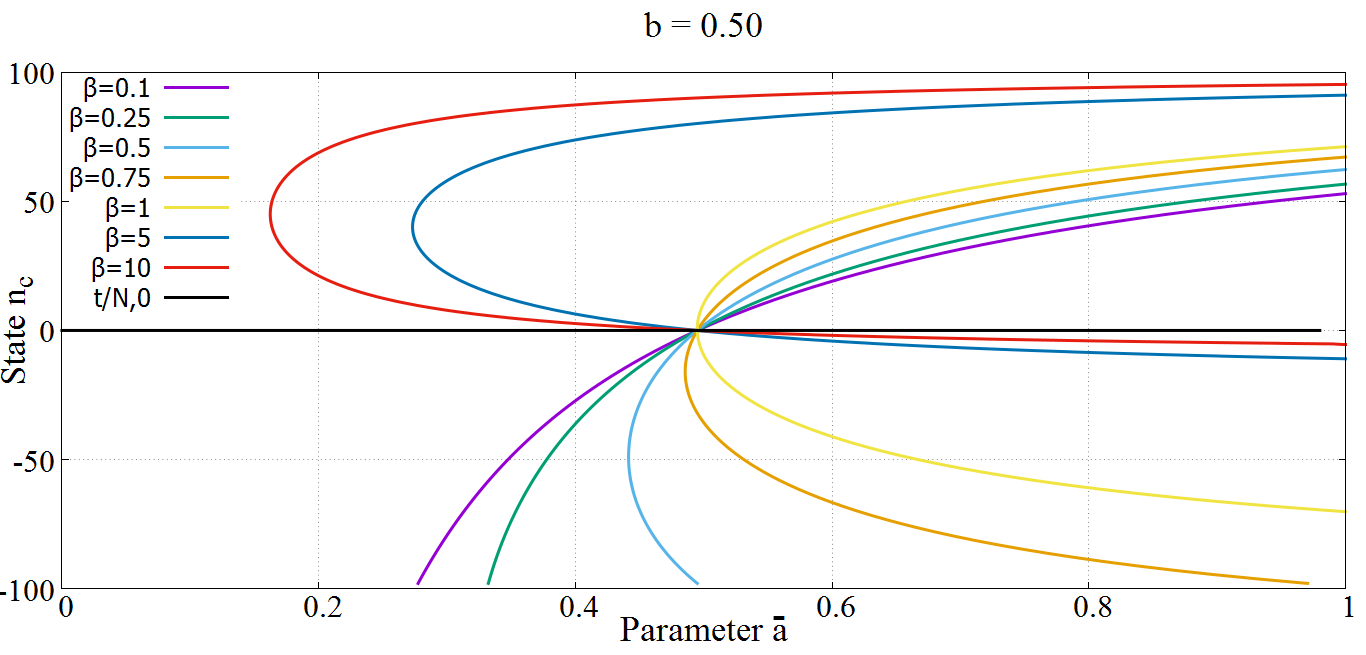
\includegraphics[width=\linewidth]{images/appendix/phaseSpace/5.png}
\end{figure}

\begin{figure}[h!]
 \centering
  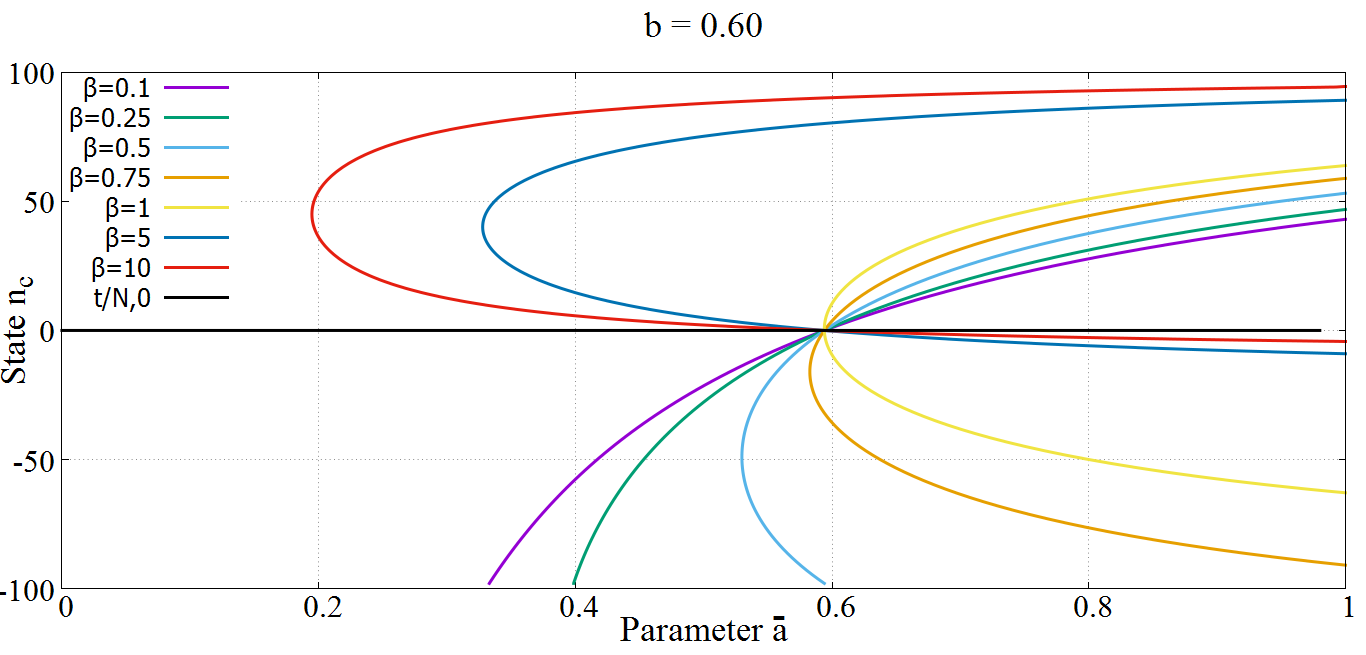
\includegraphics[width=\linewidth]{images/appendix/phaseSpace/6.png}
\end{figure}
\newpage
\begin{figure}[h!]
 \centering
  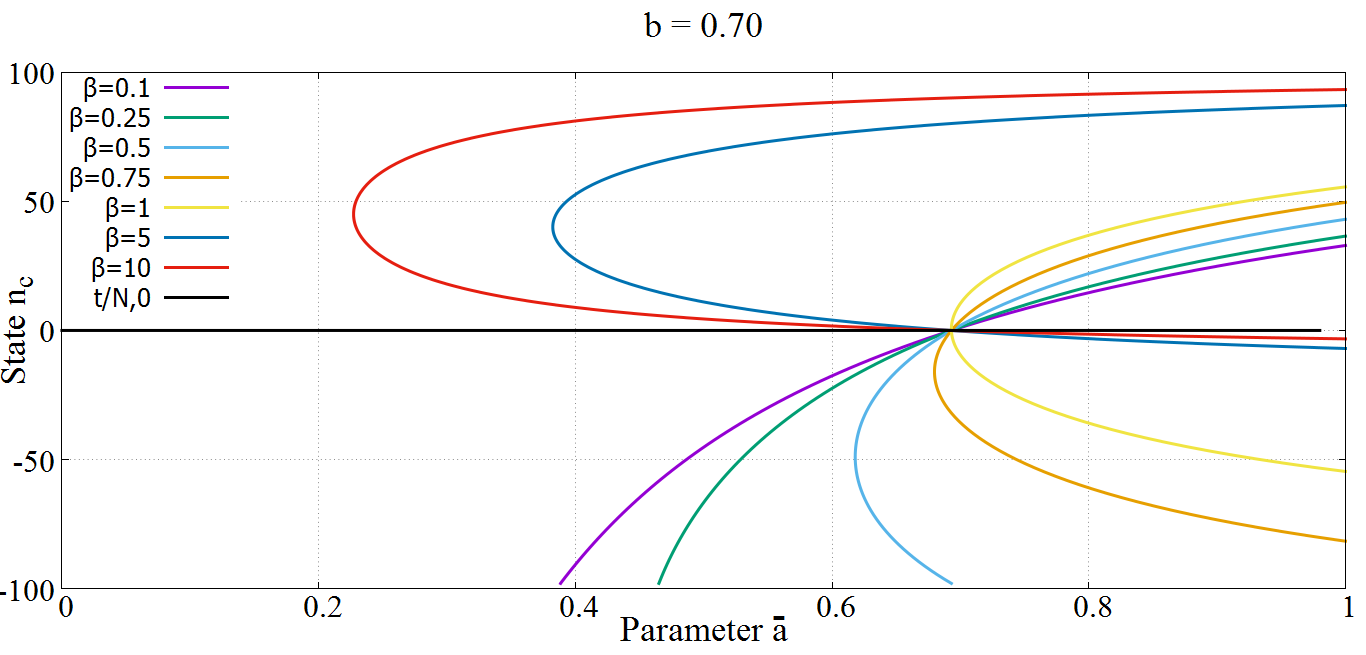
\includegraphics[width=\linewidth]{images/appendix/phaseSpace/7.png}
\end{figure}

\begin{figure}[h!]
 \centering
  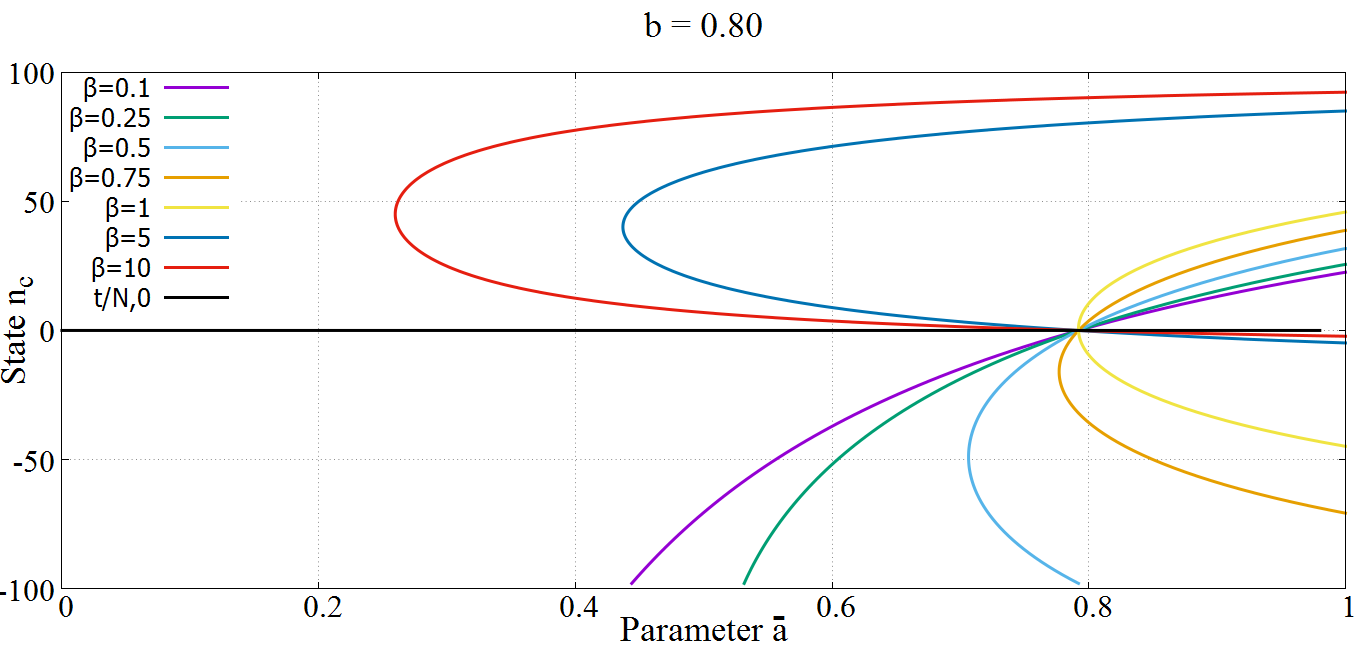
\includegraphics[width=\linewidth]{images/appendix/phaseSpace/8.png}
\end{figure}
\newpage
\begin{figure}[h!]
 \centering
  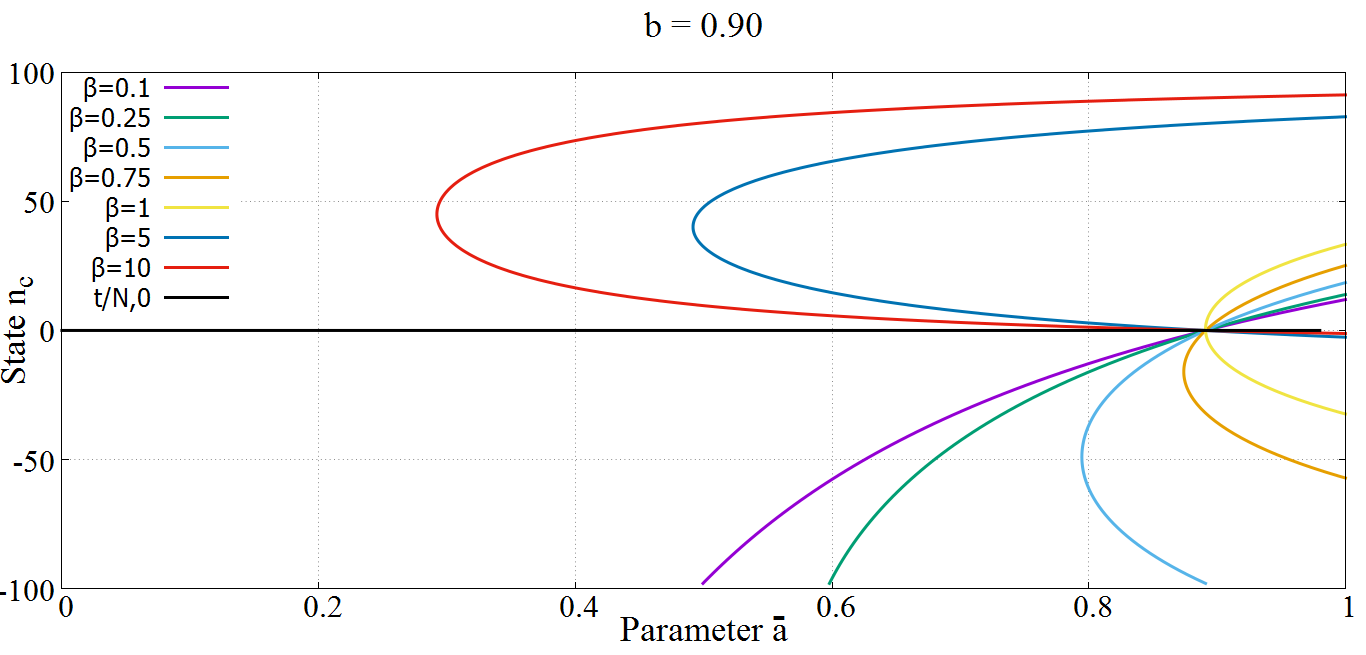
\includegraphics[width=\linewidth]{images/appendix/phaseSpace/9.png}
\end{figure}

\begin{figure}[h!]
 \centering
  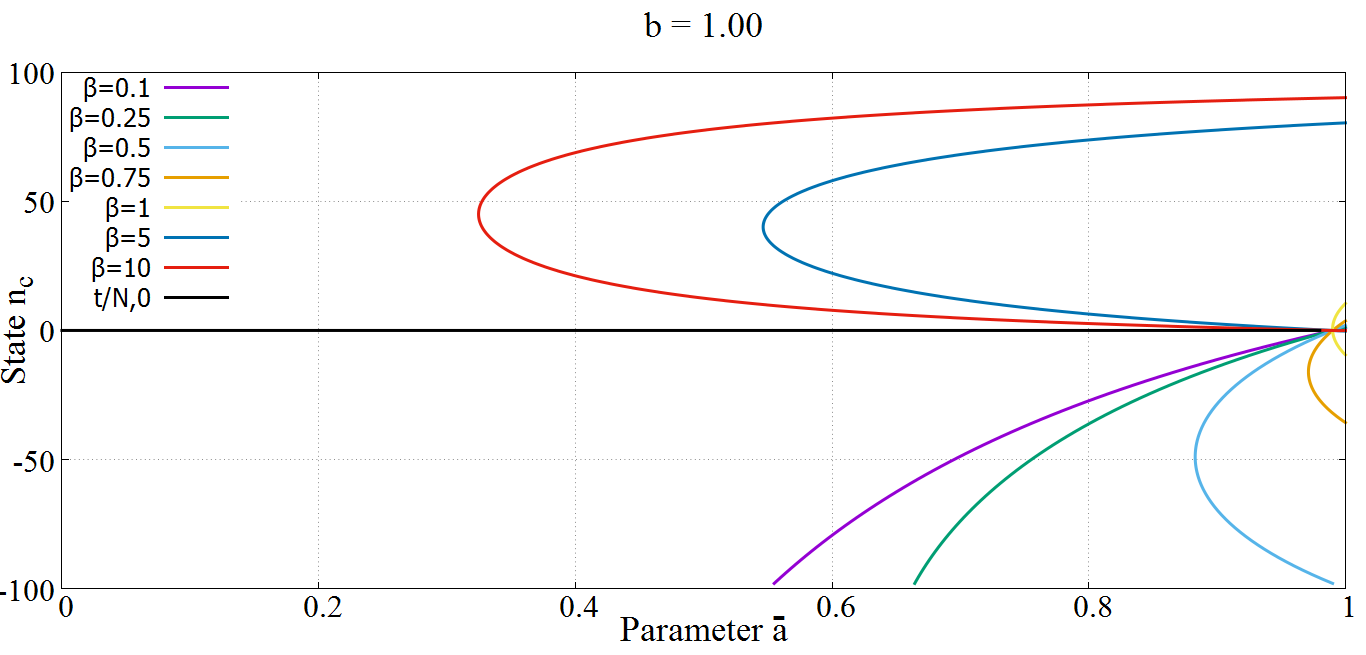
\includegraphics[width=\linewidth]{images/appendix/phaseSpace/10.png}
\end{figure}

\newpage
\section{Critical points}
\label{apndx:crita1}
\hspace{\parindent} Setting $n_{c} = 0$ in the steady-state equation \eqref{eq:steadystate} gives us this critical point of intersection

\begin{eqnarray}
\bar{a}(N-n_{c})(N-1 + \beta n_{c}) &&= b(N-1)^{2} \\
\bar{a}N(N-1) &&= b(N-1)^{2} \\
\bar{a} &&= \frac{b(N-1)^{2}}{N(N-1)} \\
\bar{a}_{1} &&= \frac{b(N-1)}{N} \\
\end{eqnarray}

On the other hand, $\bar{a_{2}}$ is arrived by plugging in a special $n_{c}$ value, $n_{c}^{*} \equiv [1+(\beta-1)N]/2\beta$.

\begin{eqnarray}
\bar{a}(N-n_{c}^{*})(N-1 + \beta n_{c}^{*}) &&= b(N-1)^{2} \\
\bar{a}_{2} &&= \frac{b(N-1)^{2}}{(N-n_{c}^{*})(N-1 + \beta n_{c}^{*})}
\end{eqnarray}

\newpage
\section{Steady-state Simulations}
\label{apndx:steadstatesim}
Shown is the code that outputs the simulations with the analytical steady-state as well as the mean of the system for a single set of parameters.

\begin{lstlisting}

#####################################################
#Simulates applause for a specific set of parameters#
#Displays the appropriate steady state value        #
#Parameters can be adjusted accordingly below       #
#####################################################


import applause_functions as app
import matplotlib.pyplot as plt
import numpy as np

N = 10
M = 10
population = N * M
time = 500
t_1 = 2
C = 0
aStoC = 1
bCtoS = 0.8
alpha = 0.6
beta = 1

fig = plt.figure()
ax = fig.add_subplot(111)
sim = app.app_sim(aStoC, bCtoS, alpha, beta, N, M, C, time, t_1)
plt.plot(sim)
ax.text(0.45*time,1,'Steady-state:'+str(round(app.steady_nC(aStoC, bCtoS, alpha, beta, population, 1),0)), fontsize=20)
ax.text(0.45*time,10,'Mean: '+str(round(np.mean(sim),1))+'$\pm$'+str(round(np.std(sim),2)), fontsize=20)
ax.text(10,100,'N = '+str(population), fontsize=15)
plt.axhline(np.mean(sim), color = 'r')
plt.axhline(app.steady_nC(aStoC, bCtoS, alpha, beta, population, 1), color = 'g')
plt.title('$a = $'+str(aStoC)+' $b = $'+str(bCtoS)+r' $\alpha=$'+str(alpha)+r' $\beta=$'+str(beta),fontsize=20)
plt.xlabel('Time',fontsize=18)
plt.ylabel('State'+r' $n_{c}$',fontsize=18)
plt.xlim(0,time)
plt.ylim(0,110)
plt.savefig('ssB.png')
plt.show()

\end{lstlisting}

Following is the code used to generate the data points of the simulated steady-state values to be plotted against the analytic steady-state solutions.

\begin{lstlisting}

#Takes the last point of the simulation (Trials) times then calculates mean and std#
#Does so for varying a-bar values                                                  #
#Creates .csv file with columns: a-bar, mean, std                                  #
#Plots the data points                                                             #
#Parameters can be adjusted accordingly below                                      #


import applause_functions as app
import matplotlib.pyplot as plt
import numpy as np

#####Simulation Parameters#####
N = 10
M = 10
startPop = 20
time = 100
t_1 = 0
aStoC = 1.0
bCtoS = 0.8 
alpha = 1
beta = 10
###Point Generator Parameters###
Trials = 50
interval = 0.02
##############################
def pointGen(aStoC, bCtoS, beta, N, M, startPop, time, t_1, Trials, interval):
    
    meanlist = []
    stdlist = []
    ilist = []
    for i in np.arange(0,1.0,interval):
        list_a = []
        for j in range(Trials):
            list_a.append(app.app_sim(aStoC, bCtoS, i, beta, N, M, startPop, time, t_1)[time-1]) #takes the last number from the appsim vector
        mean = np.mean(np.array(list_a))
        std = np.std(np.array(list_a))  
        meanlist.append(mean)
        stdlist.append(std)
        ilist.append(i)

    ilist = np.array(ilist)
    meanlist = np.array(meanlist)
    stdlist = np.array(stdlist)
    
    #writes ilist,meanlist, and stdlist into a txt file
    filename = 'b = ' + str(bCtoS) + ', beta = ' + str(beta) + ', startPop = ' + str(startPop) + '.txt'    
    with open(filename,'w') as f:
        lis=[ilist,meanlist,stdlist]
        for x in zip(*lis):
            f.write("{0}\t{1}\t{2}\n".format(*x))
            
    return (ilist,meanlist,stdlist)
\end{lstlisting}

\newpage
\section{Steady-state Simulations Results}
\label{apndx:ssexpt}
Shown are the phase space plots along with the simulated data points using the same parameters for various $b$ and $\beta$ values.

\begin{figure}[h!]
 \centering
  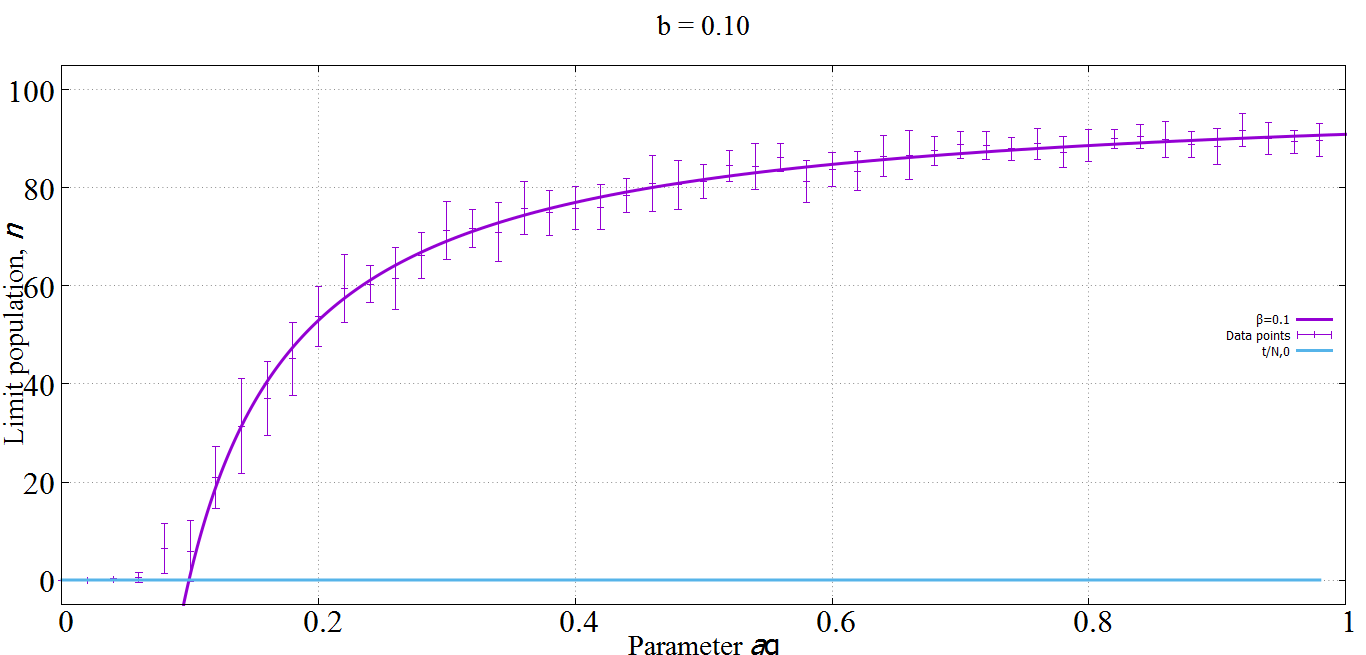
\includegraphics[width=\linewidth]{images/appendix/simexpt/1.png}
\end{figure}

\begin{figure}[h!]
 \centering
  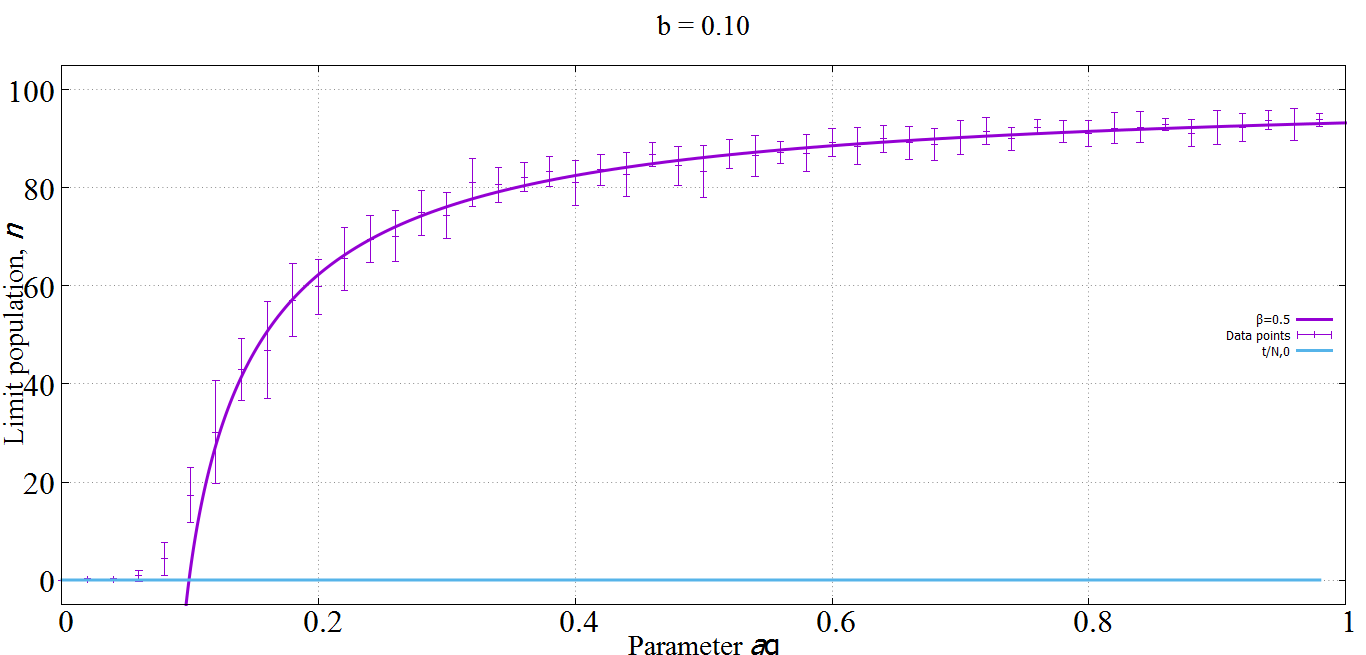
\includegraphics[width=\linewidth]{images/appendix/simexpt/2.png}
\end{figure}
\newpage
\begin{figure}[h!]
 \centering
  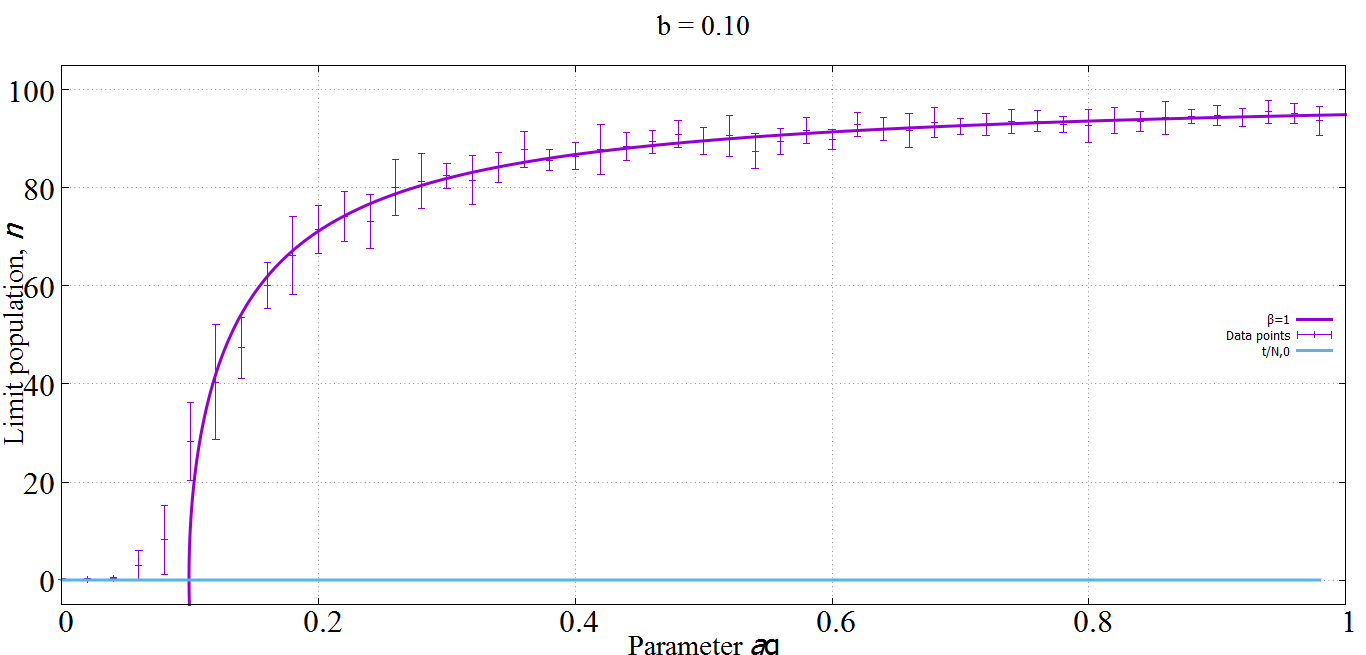
\includegraphics[width=\linewidth]{images/appendix/simexpt/3.png}
\end{figure}

\begin{figure}[h!]
 \centering
  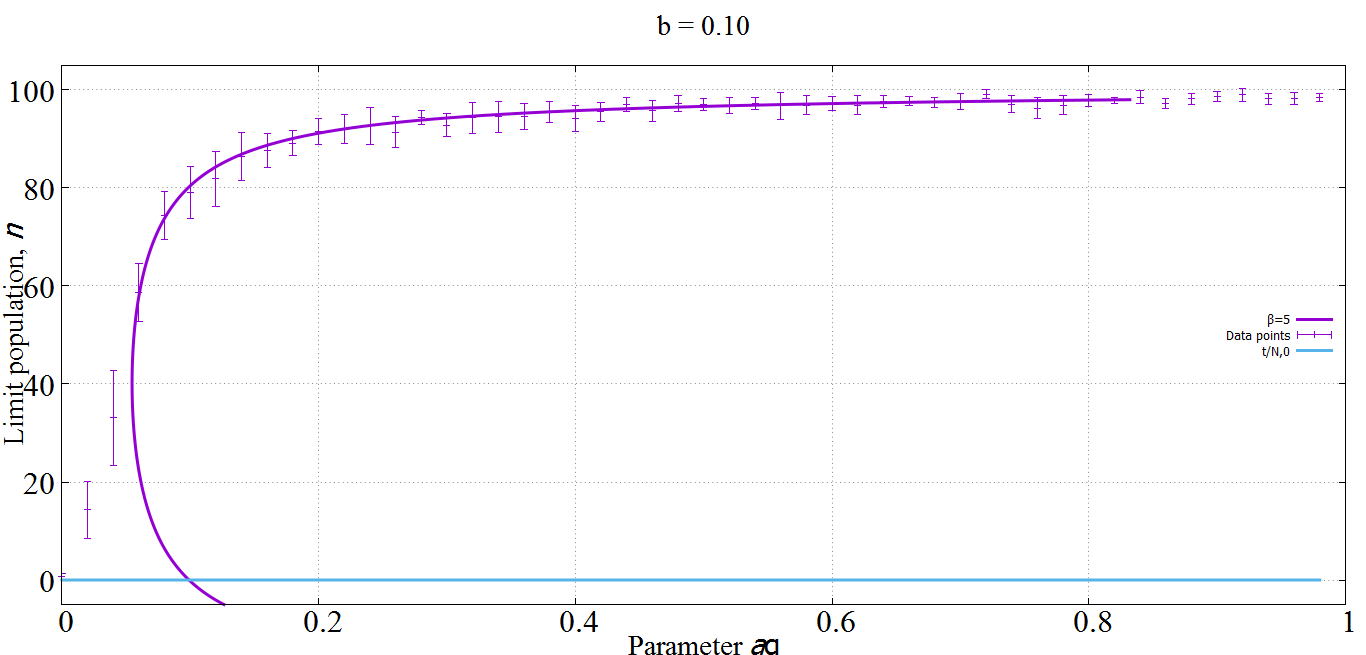
\includegraphics[width=\linewidth]{images/appendix/simexpt/4.png}
\end{figure}
\newpage
\begin{figure}[h!]
 \centering
  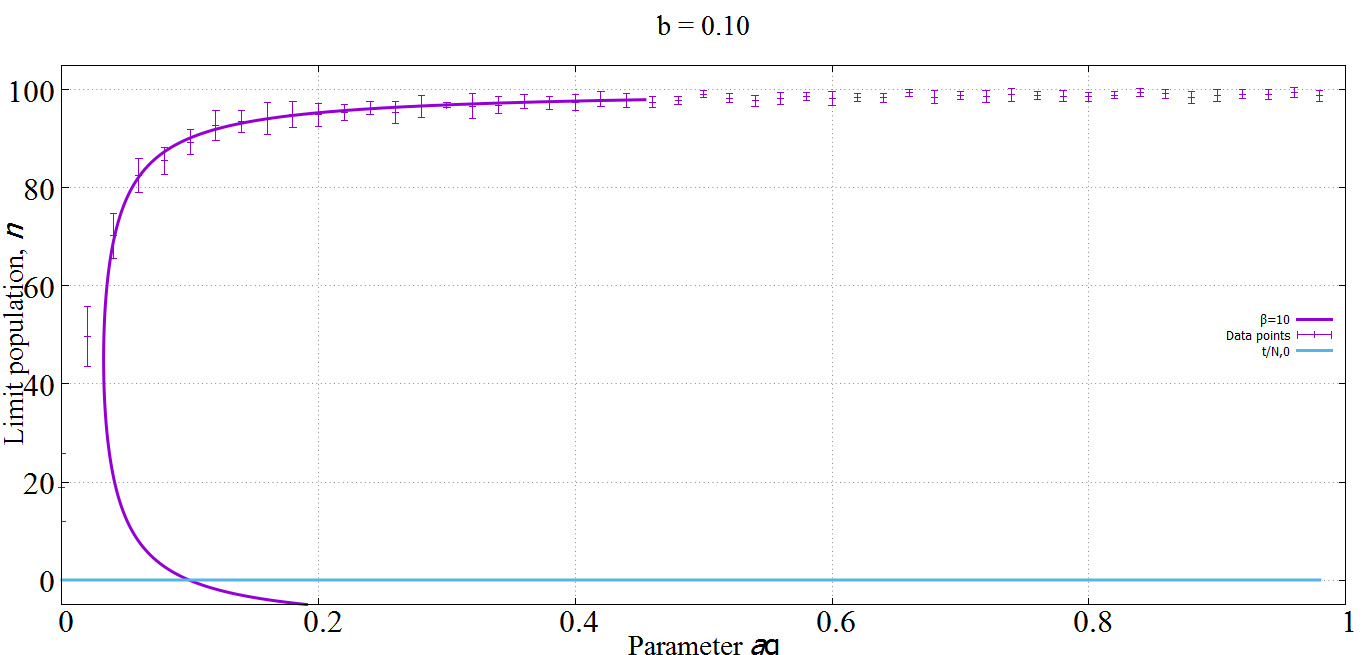
\includegraphics[width=\linewidth]{images/appendix/simexpt/5.png}
\end{figure}

\begin{figure}[h!]
 \centering
  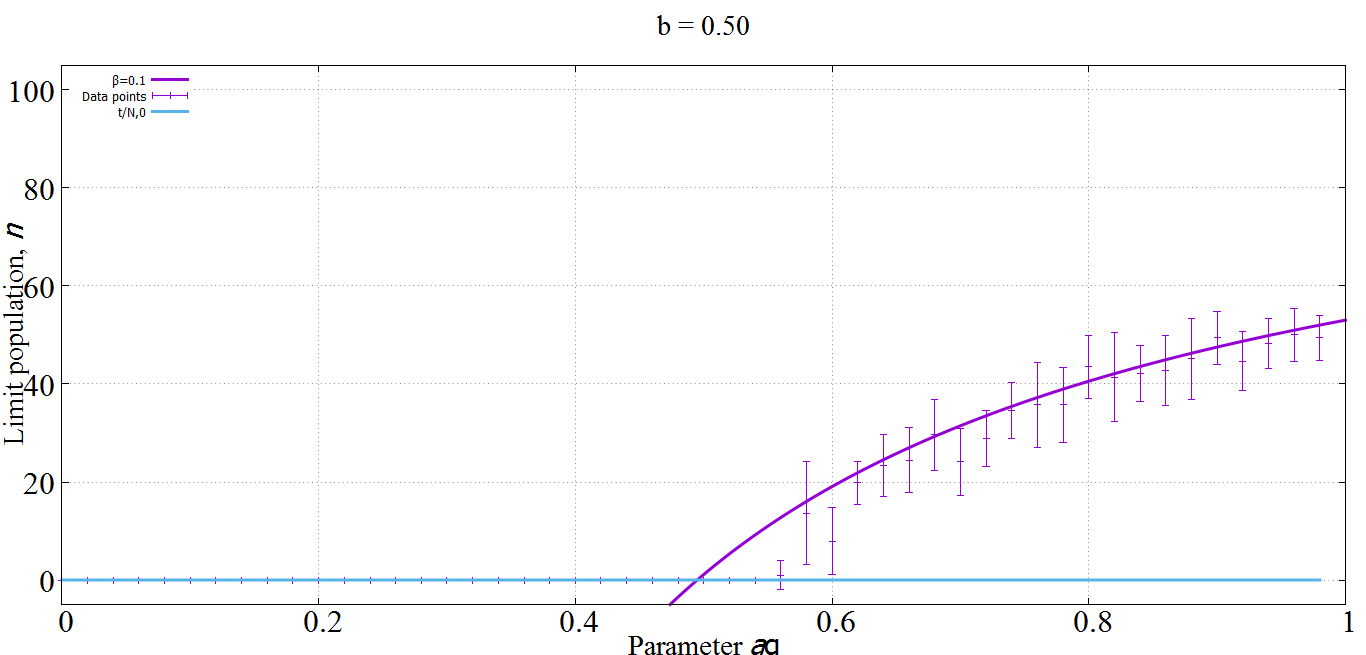
\includegraphics[width=\linewidth]{images/appendix/simexpt/6.png}
\end{figure}
\newpage
\begin{figure}[h!]
 \centering
  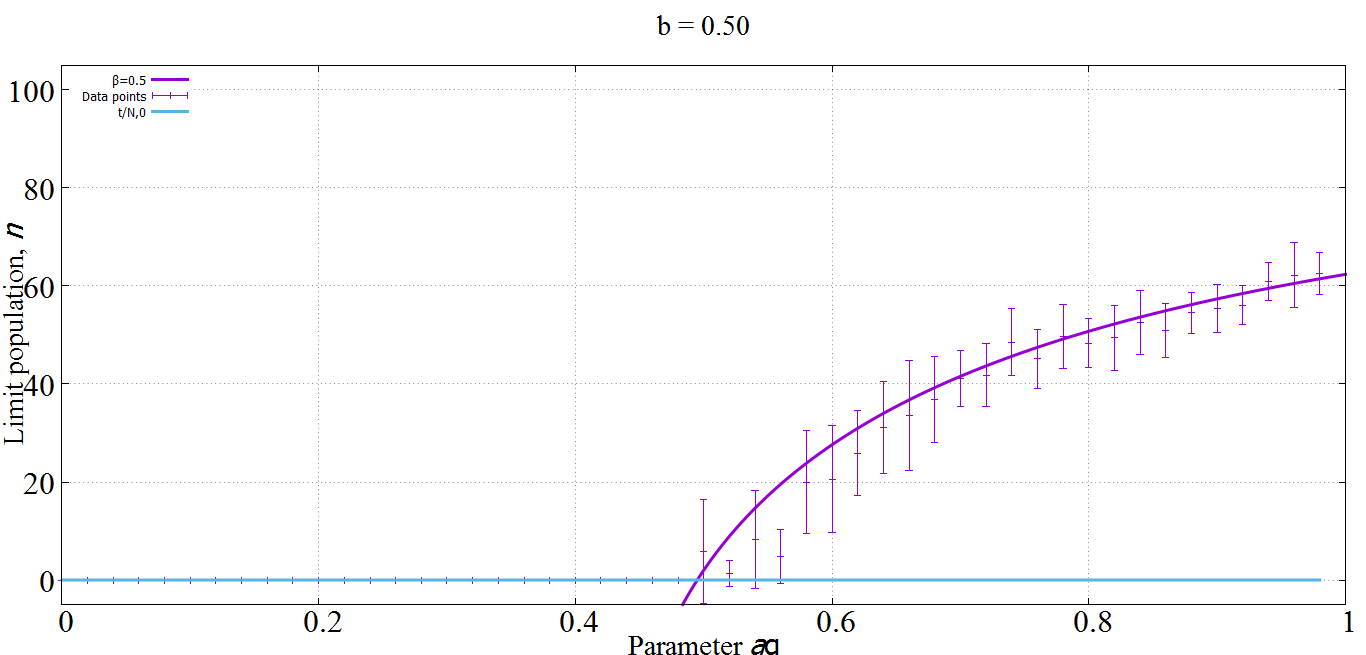
\includegraphics[width=\linewidth]{images/appendix/simexpt/7.png}
\end{figure}

\begin{figure}[h!]
 \centering
  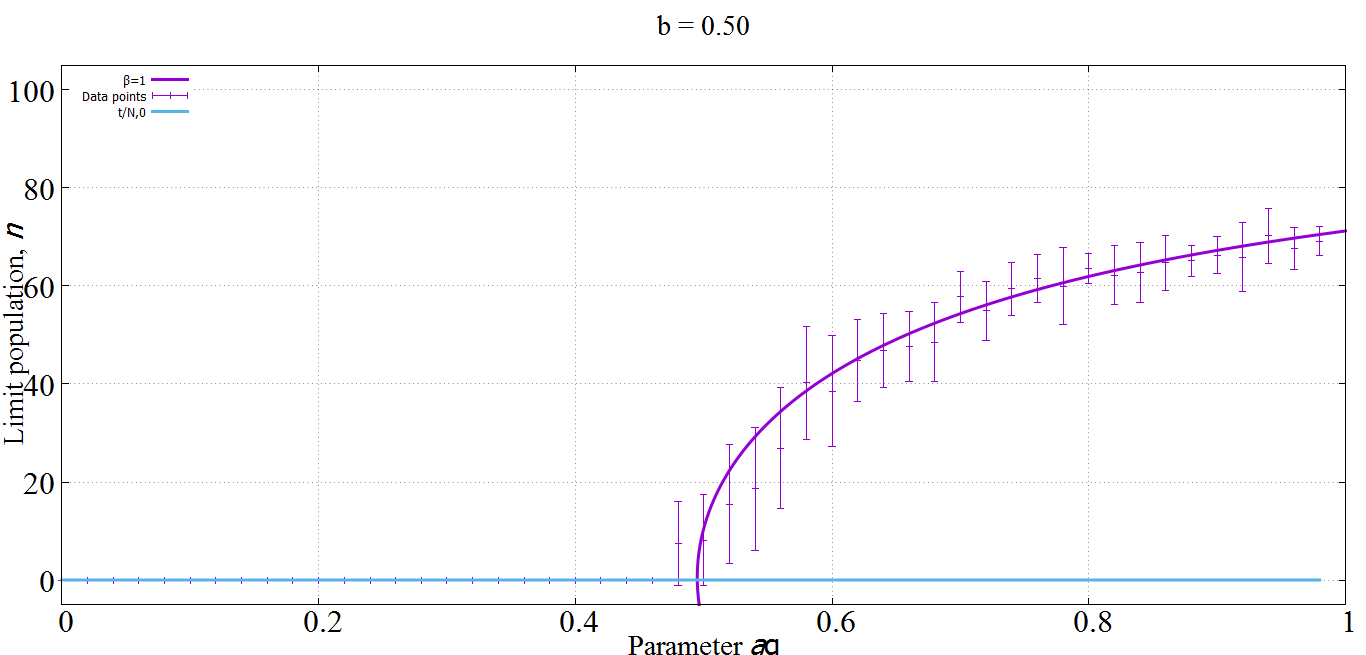
\includegraphics[width=\linewidth]{images/appendix/simexpt/8.png}
\end{figure}
\newpage
\begin{figure}[h!]
 \centering
  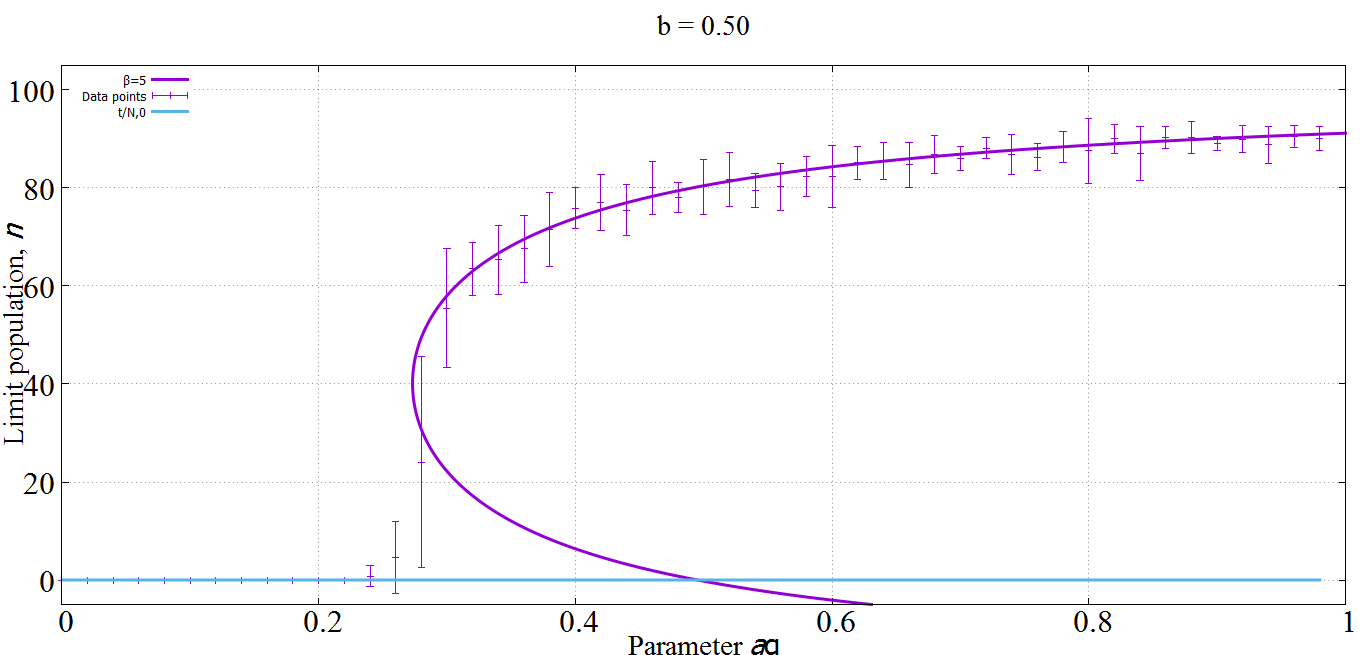
\includegraphics[width=\linewidth]{images/appendix/simexpt/9.png}
\end{figure}

\begin{figure}[h!]
 \centering
  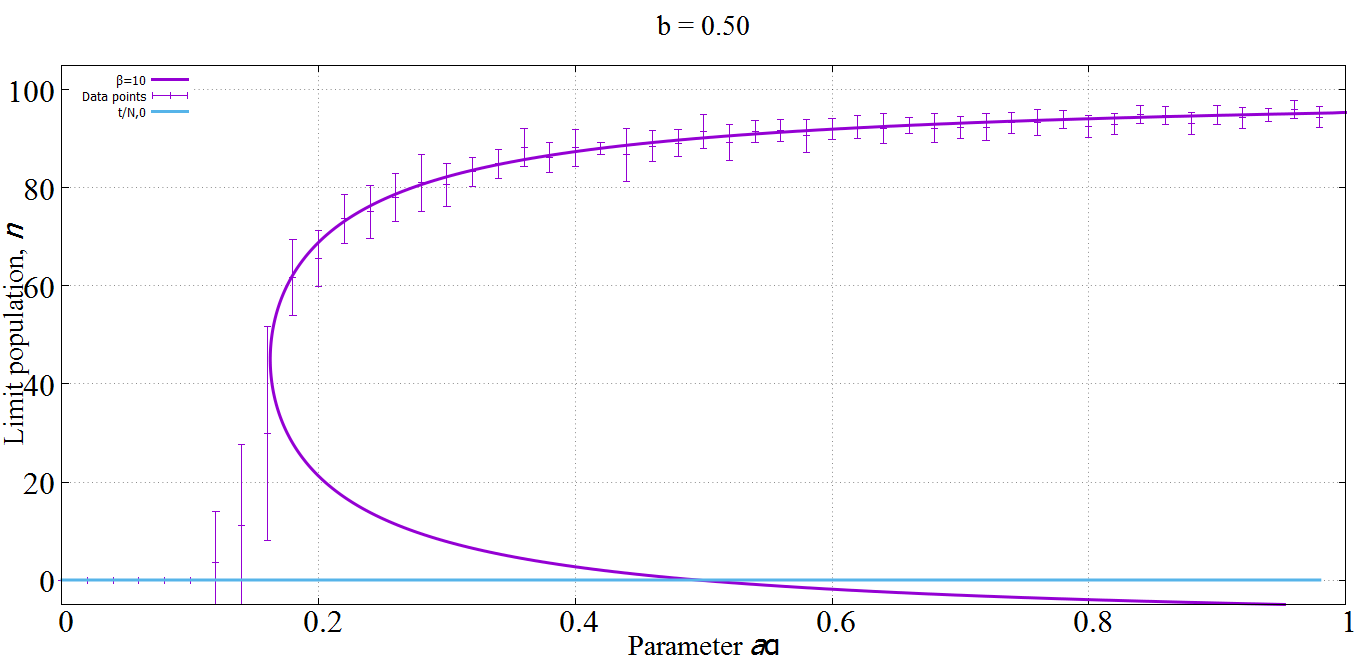
\includegraphics[width=\linewidth]{images/appendix/simexpt/10.png}
\end{figure}
\newpage
\begin{figure}[h!]
 \centering
  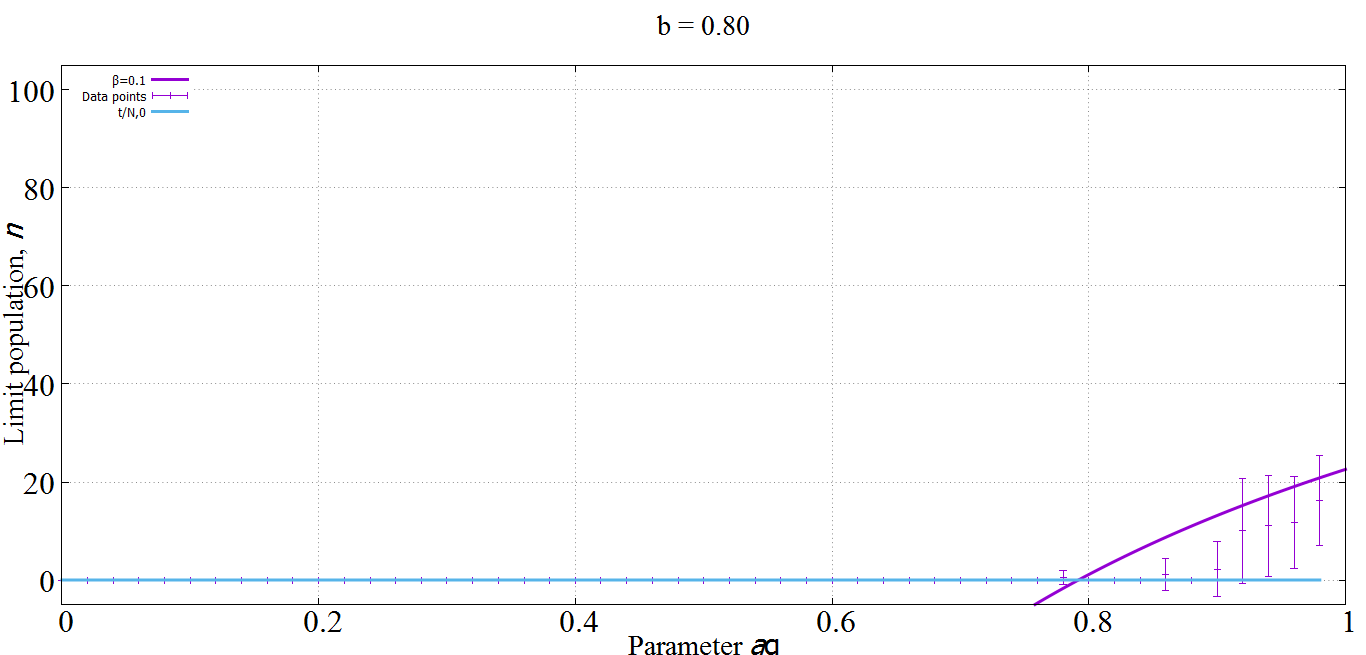
\includegraphics[width=0.6\linewidth]{images/appendix/simexpt/11.png}
\end{figure}

\begin{figure}[h!]
 \centering
  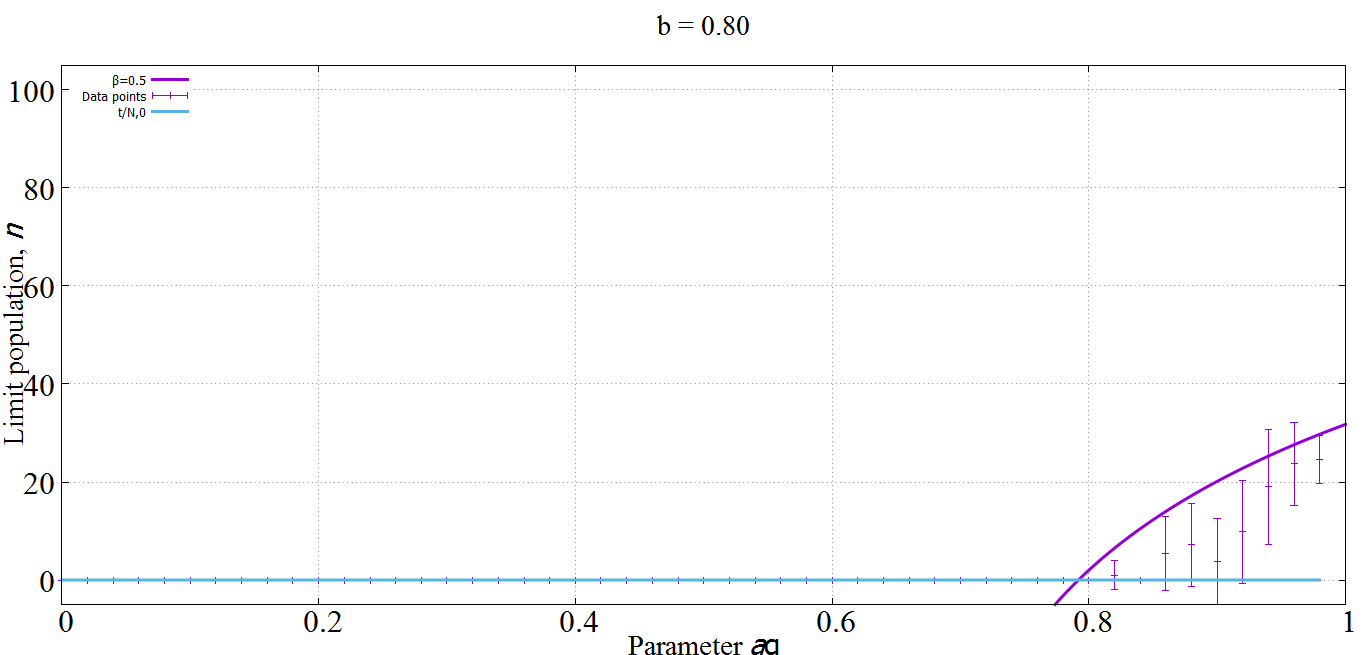
\includegraphics[width=0.6\linewidth]{images/appendix/simexpt/12.png}
\end{figure}

\begin{figure}[h!]
 \centering
  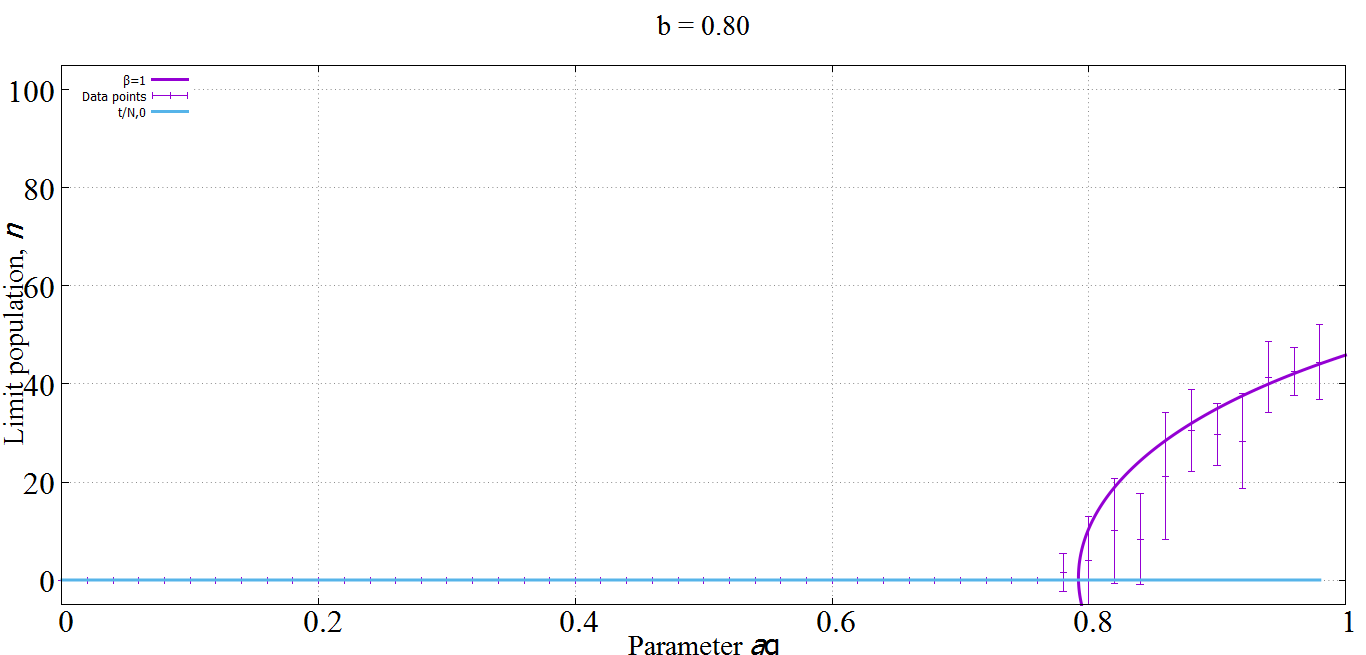
\includegraphics[width=0.6\linewidth]{images/appendix/simexpt/13.png}
\end{figure}
\newpage
\begin{figure}[h!]
 \centering
  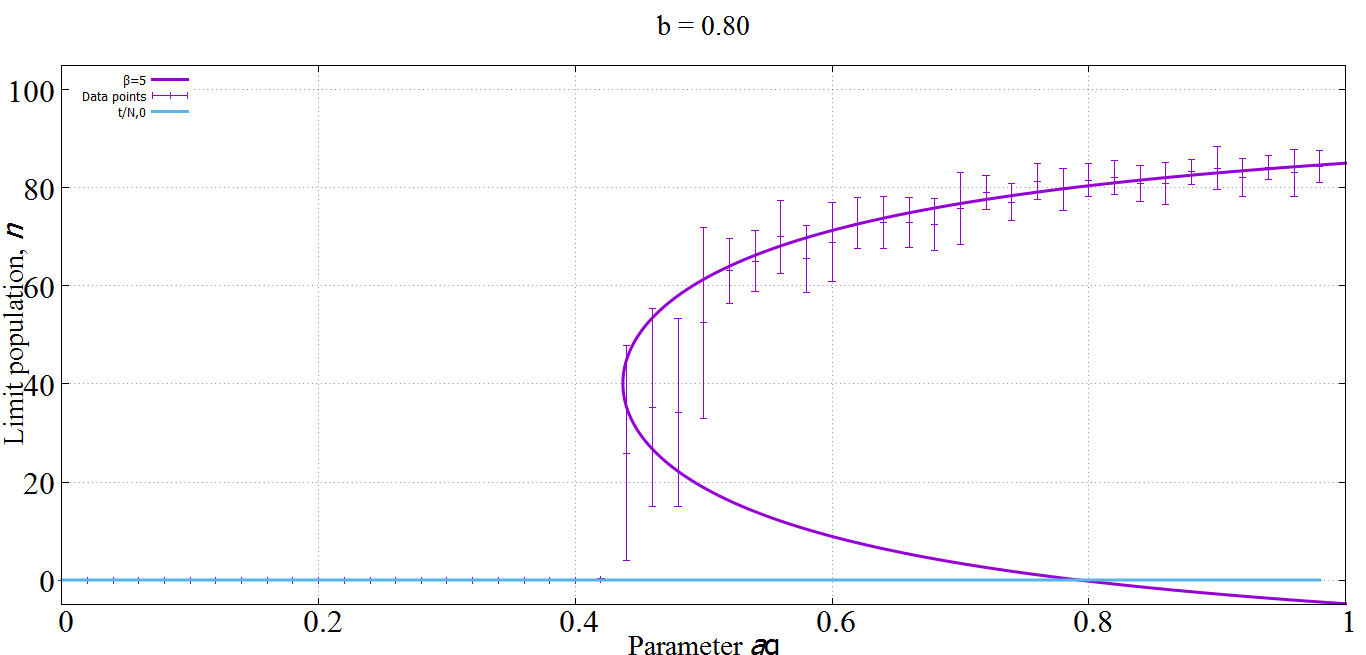
\includegraphics[width=\linewidth]{images/appendix/simexpt/14.png}
\end{figure}

\begin{figure}[h!]
 \centering
  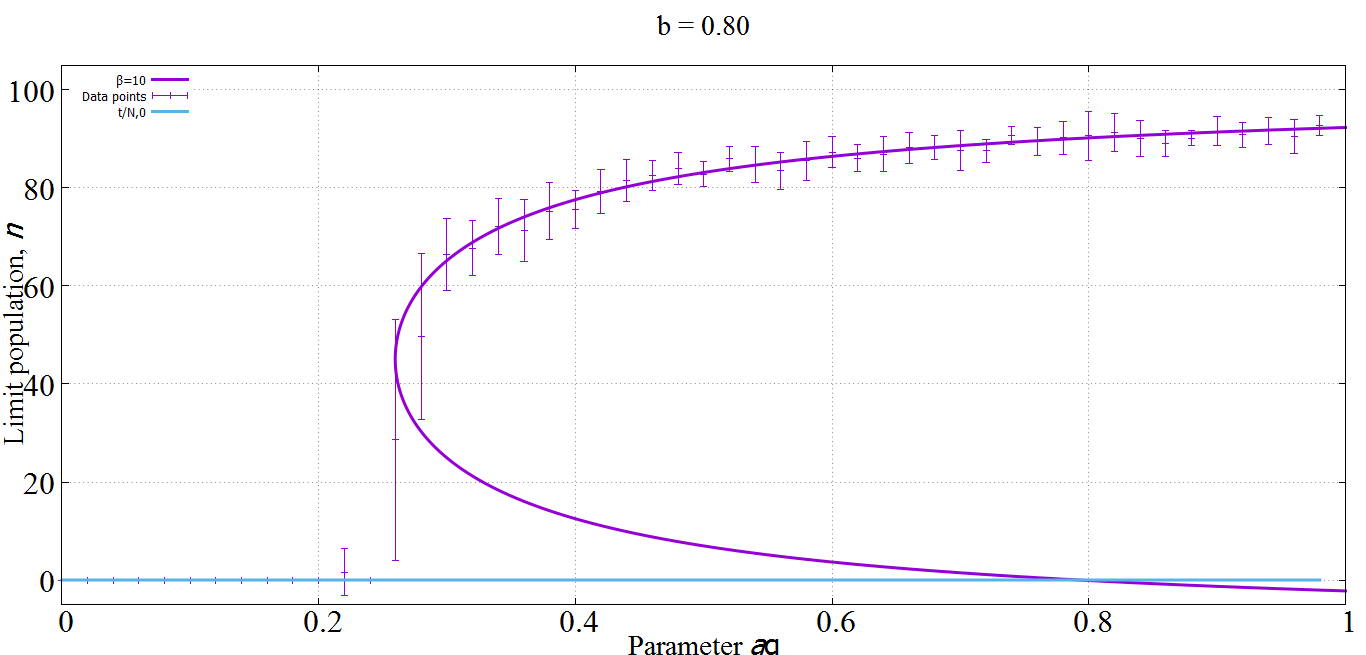
\includegraphics[width=\linewidth]{images/appendix/simexpt/15.png}
\end{figure}

\newpage
\section{Vector Generator}
\label{apndx:vectsim}

Following is the code used to generate the vectors pointing to the steady-state given the initial to be plotted against the analytic steady-state solutions.

\begin{lstlisting}
import applause_functions as app
import matplotlib.pyplot as plt
import numpy as np
import time as t

speed = t.clock()

N = 10
M = 10
startPop = 1
time = 100
t_1 = 0
aStoC = 1.0
bCtoS = 0.8 
alpha = 1
beta = 10

x = 11
y = 11
z = 100

#a = app.app_sim(aStoC, bCtoS, alpha, beta, N, M, startPop, time, t_1)

def probFilter(a): #converts all non-zero values in a list to 1
    for q in range(len(a)):
        if a[q] != 0:
            a[q] = 1

def lastList(abar, bCtoS, alpha, beta, N, M, start, time, t_1, iter): 
    #runs app_sim 'iter' times and lists the last element per iteration
    finalVal = []
    probVal = []
    for i in range(iter):
        x = app.app_sim(abar, bCtoS, alpha, beta, N, M, start, time, t_1)[-1]
        finalVal.append(x)
        if x==0:
            probVal.append(0.0)
        else:
            probVal.append(1.0)
    return finalVal, probVal
    
    
def heatData(bCtoS, beta, x, y, z):
    abarRange = np.linspace(0,1,x)
    startRange = np.linspace(0,100,y)  
    
    n = 0
    
    abar = np.zeros(len(abarRange)*len(startRange))
    start = np.zeros(len(abarRange)*len(startRange))
    rawHeat = np.zeros(len(abarRange)*len(startRange))
        
    for i in range(len(abarRange)):
        for j in range(len(startRange)):
            k = lastList(abarRange[i], bCtoS, alpha, beta, N, M, startRange[j], time, t_1, z)
            abar[n] = (abarRange[i])
            start[n] = (startRange[j])
            rawHeat[n] =(sum(k[1])/len(k[1]))
            n += 1
            print(t.clock() - speed)
            
    
    filename = 'b = ' + str(bCtoS) + ', beta = ' + str(beta) + ', x = ' + str(x) + ', y = ' + str(y) + ', z = ' + str(z) + '.txt'    
    with open(filename,'w') as f:
        lis=[abar,start,rawHeat]
        for x in zip(*lis):
            f.write("{0}\t{1}\t{2}\n".format(*x))        
            
    return abar,start,rawHeat
\end{lstlisting}

\newpage
\section{Vector Graphs}
\label{apndx:vectgraph}
Shown are the phase space plots along with probabilistic vectors pointing towards the steady-state for various $b$ and $\beta$ values.

\begin{figure}[h!]
 \centering
  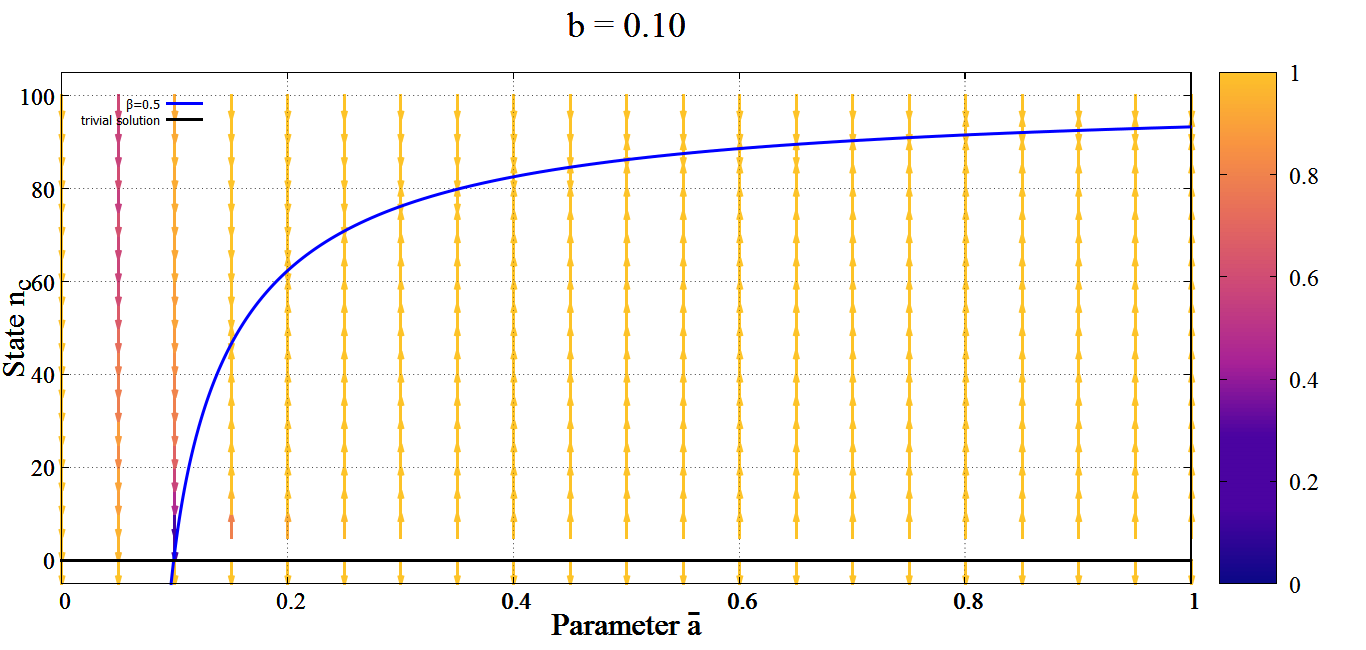
\includegraphics[width=\linewidth]{images/appendix/vectors/1.png}
\end{figure}

\begin{figure}[h!]
 \centering
  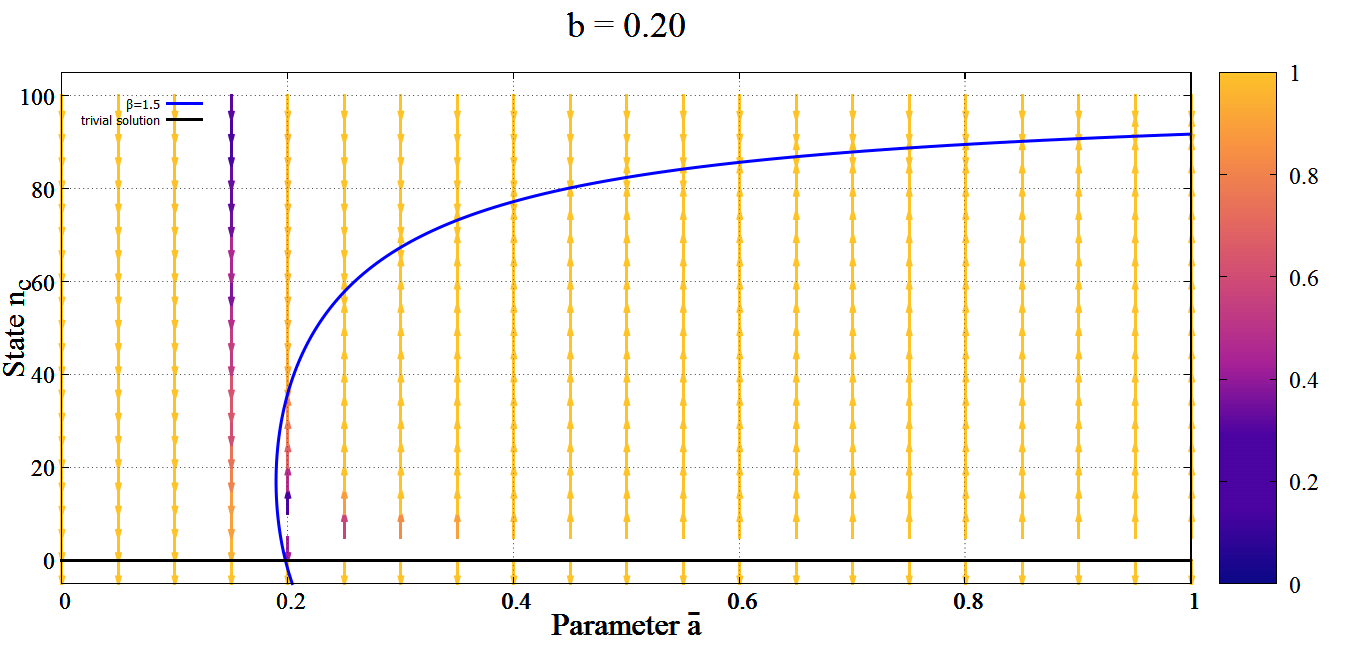
\includegraphics[width=\linewidth]{images/appendix/vectors/2.png}
\end{figure}
\newpage
\begin{figure}[h!]
 \centering
  \includegraphics[width=\linewidth]{images/appendix/vectors/3.png}
\end{figure}

\begin{figure}[h!]
 \centering
  \includegraphics[width=\linewidth]{images/appendix/vectors/5.png}
\end{figure}

\newpage
\section{Simulations Spatial Effects}
\label{apndx:spacesim}

Shown is the code from the library that incorporates spatial effects to the simulations.

\begin{lstlisting}
#spatial-dependent feedack, you can control the 'radius' of the reference agent
#taper refers to how many to add at the ends;radius = 0 taper = 1 is '90deg'    
def feedback_space(alpha,system,system_row, system_column, N, M, radius, taper):
    applause_state = []
    for i in range(system_row):
        radius_mech = 0
        applause_state.append(system[i,system_column])
        while radius_mech != radius + taper*(system_row - i):
            radius_mech += 1
            if system_column + radius_mech < M:
                applause_state.append(system[i,system_column + radius_mech])
            if system_column - radius_mech > -1:
                applause_state.append(system[i,system_column - radius_mech])
    return alpha*nan_to_num(sum(applause_state)/len(applause_state))
    
def feedback_180deg(alpha,system,system_row, M): #reverted to simpler feedback space functions since runs took too long
    applause_state = [0]
    for i in range(system_row):
        applause_state.append(sum(system[i]))
    return alpha*nan_to_num(sum(applause_state)/(system_row*M))
    
def feed_space(aStoC, bCtoS, alpha, beta, N, M, C, t, t_1,radius,taper):
    population = N * M
    AGENT = audience(N, M, C)
    graph = []
    zeroCount = 0

    for k in range(t):
        nC = sum(AGENT) #number of people clapping
        if nC == 0:
            zeroCount += 1
        graph.append(nC)
        for i in range(N):
            for j in range(M):
                if AGENT[i,j] == 0:
                    if random() <= aStoC * (1 - (1-force_func(k, t_1)) * (1 - feedback_space(alpha,AGENT,i, j, N, M, radius, taper))):
                        AGENT[i,j] += 1
                else:
                    if random() <= bCtoS * feedback_beta(beta, nC, population):
                        AGENT[i,j] -= 1
        if zeroCount == 6:
            break
            return graph
    return graph

#sim with spatial dependence specific to 180 deg
def sim_space(aStoC, bCtoS, alpha, beta, N, M, C, t, t_1):
    population = N * M
    AGENT = audience(N, M, C)
    graph = []
    zeroCount = 0

    for k in range(t):
        nC = sum(AGENT) #number of people clapping
        if nC == 0:
            zeroCount += 1
        graph.append(nC)
        for i in range(N):
            for j in range(M):
                if AGENT[i,j] == 0:
                    if random() <= aStoC * (1 - (1-force_func(k, t_1)) * (1 - feedback_180deg(alpha,AGENT,i, M))):
                        AGENT[i,j] += 1
                else:
                    if random() <= bCtoS * feedback_beta(beta, nC, population):
                        AGENT[i,j] -= 1
        if zeroCount == 6:
            break
            return graph
    return graph        
\end{lstlisting}

Shown is the code used to compare the different feedback functions.

\begin{lstlisting}
import applause_functions as app
import matplotlib.pyplot as plt
import numpy as np
import time

N = 10
M = 10
population = N * M
t = 500
t_1 = 1
C = 0
aStoC = 0.7
bCtoS = 0.8
alpha = 0.5
beta = 4

start_time = time.time()

fig = plt.figure()
ax = fig.add_subplot(111)
sim1 = app.app_sim(aStoC, bCtoS, alpha, beta, N, M, C, t, t_1)
sim2 = app.feed_space(aStoC, bCtoS, alpha, beta, N, M, C, t, t_1,M,0)
sim3 = app.feed_space(aStoC, bCtoS, alpha, beta, N, M, C, t, t_1,0,1)
sim4 = app.feed_space(aStoC, bCtoS, alpha, beta, N, M, C, t, t_1,0,0)
plt.plot(sim1, color='b', label="FC")
plt.plot(sim2, color='r', label="180deg")
plt.plot(sim3, color='g', label="90deg")
plt.plot(sim4, color='y', label="0deg")
plt.legend(loc=4)

ax.text(1,5,'N = '+str(population), fontsize=15)

plt.title('$a = $'+str(aStoC)+' $b = $'+str(bCtoS)+r' $\alpha=$'+str(alpha)+r' $\beta=$'+str(beta),fontsize=20)
plt.xlabel('Time',fontsize=18)
plt.ylabel('State'+r' $n_{c}$',fontsize=18)
plt.xlim(0,30)
plt.ylim(0,110)
plt.savefig('feedback_sim7.png')
plt.show()
#print(sim2)
#print(str(time.time() - start_time) + ' seconds')
\end{lstlisting} 

\newpage
\section{Investigating Population Dependence}
\label{apndx:popdep}
Shown is the code used to investigate if the applause duration is dependent on population size.

\begin{lstlisting}
import applause_functions as app
import matplotlib.pyplot as plt
import numpy as np
import time

N = 10
M = 10
population = N * M
t = 60
t_1 = 2
C = 0
aStoC = 1
bCtoS = 0.8
alpha = 0.2
beta = 1

start_time = time.time()
trials = 5
popSet = [4,5,6,7,8,9,10,15,18,20,25,28,32,54,70,86,100,159]#,223,274,315] #set sqrt numbers that encompass the log scale

#used to take the index for which SIM becomes 0; gets the applause duration
def indexFilter(value,qlist,r1,r2):
    try:
        return qlist.index(value,r1,r2)
    except ValueError:
        return 0

for alpha_iter in range(8,11,1):
    for bCtoS_iter in range(1,11,1):
        
        #lists to be graphed
        duration = []
        durationSTD = []
        population = []
        
        for pop in popSet: #goes thru popSet
            appDurationTrials = [] #temporary holder of trials to be averaged   
            for j in range(trials): #simulates parameters and population TRAIL times
                N = pop
                sim = app.sim_space(aStoC, bCtoS_iter*0.1, alpha_iter*0.1, beta, N, N, C, t, t_1)
                if indexFilter(0,sim,1,t) != 0:
                    appDurationTrials.append(indexFilter(0,sim,1,t))
                    print('Trial ' + str(j) + ' complete '  + str(time.strftime("%Y-%m-%d %H:%M:%S")))
                else:
                    appDurationTrials.append(indexFilter(0,sim,1,t))
                    print('Trial ' + str(j) + ' reached non-zero steady state '  + str(time.strftime("%Y-%m-%d %H:%M:%S")))
                    break
        
            duration.append(np.mean(appDurationTrials))
            durationSTD.append(np.std(appDurationTrials))
            population.append(N*N)
            print("Population " + str(pop) + " complete " + str(time.strftime("%Y-%m-%d %H:%M:%S")))
        #scatter plot with error bars
        #plt.subplot(111, xscale="log")
        fig = plt.figure()
        ax = fig.add_subplot(111,xscale="log") 
        x = population 
        y = duration 
        plt.errorbar(x, y, xerr=0, yerr=durationSTD, fmt='o') 
        plt.title('$a = $'+str(aStoC)+' $b = $'+str(round(bCtoS_iter*0.1,1))+r' $\alpha=$'+str(round(alpha_iter*0.1,1))+r' $\beta=$'+str(beta),fontsize=20)
        plt.xlabel('Size',fontsize=18)
        plt.ylabel('Time',fontsize=18)
        plt.savefig('a = '+str(aStoC)+' b = '+str(round(bCtoS_iter*0.1,1))+r' alpha='+str(round(alpha_iter*0.1,1))+r' beta='+str(beta)+'.png')
        plt.show()
        print(str(time.time() - start_time) + ' seconds; ' + str(time.strftime("%Y-%m-%d %H:%M:%S")))
\end{lstlisting}

\newpage
\section{Best fit parameter sets}
\label{apndx:bestfit}
Shown are the graphs of applause duration versus population size of parameter sets that closely resemble the real-life data points.

\begin{figure}[h]
  \centering
  \begin{subfigure}[b]{0.4\linewidth}
    \includegraphics[width=\linewidth]{images/appendix/bestfit/confirm1.png}
  \end{subfigure}
  \begin{subfigure}[b]{0.4\linewidth}
    \includegraphics[width=\linewidth]{images/appendix/bestfit/confirm2.png}
  \end{subfigure}
\end{figure}

\begin{figure}[h]
  \centering
  \begin{subfigure}[b]{0.4\linewidth}
    \includegraphics[width=\linewidth]{images/appendix/bestfit/confirm3.png}
  \end{subfigure}
  \begin{subfigure}[b]{0.4\linewidth}
    \includegraphics[width=\linewidth]{images/appendix/bestfit/confirm4.png}
  \end{subfigure}
\end{figure}

\begin{figure}[h]
  \centering
  \begin{subfigure}[b]{0.4\linewidth}
    \includegraphics[width=\linewidth]{images/appendix/bestfit/confirm5.png}
  \end{subfigure}
  \begin{subfigure}[b]{0.4\linewidth}
    \includegraphics[width=\linewidth]{images/appendix/bestfit/confirm6.png}
  \end{subfigure}
\end{figure}
%%more appendices can be added here.

%% Bibliography and style, include osa.bst for style...
\bibliographystyle{unsrt}
\bibliography{biblio}
\nocite{*}

%% Finishing the document...
\end{document}
